
%% Beginning of file 'sample63.tex'
%%
%% Modified 2019 June
%%
%% This is a sample manuscript marked up using the
%% AASTeX v6.3 LaTeX 2e macros.
%%
%% AASTeX is now based on Alexey Vikhlinin's emulateapj.cls 
%% (Copyright 2000-2015).  See the classfile for details.

%% AASTeX requires revtex4-1.cls (http://publish.aps.org/revtex4/) and
%% other external packages (latexsym, graphicx, amssymb, longtable, and epsf).
%% All of these external packages should already be present in the modern TeX 
%% distributions.  If not they can also be obtained at www.ctan.org.

%% The first piece of markup in an AASTeX v6.x document is the \documentclass
%% command. LaTeX will ignore any data that comes before this command. The 
%% documentclass can take an optional argument to modify the output style.
%% The command below calls the preprint style which will produce a tightly 
%% typeset, one-column, single-spaced document.  It is the default and thus
%% does not need to be explicitly stated.
%%
%%
%% using aastex version 6.3
\documentclass[twocolumn]{aastex63}
\usepackage{lineno} 
\usepackage{lipsum} %Creates example text
\linenumbers

%% The default is a single spaced, 10 point font, single spaced article.
%% There are five other style options available via an optional argument. 
%% They can be invoked like this:
%%
%% \documentclass[arguments]{aastex63}
%% 
%% where the layout options are:
%%
%%  twocolumn   : two text columns, 10 point font, single spaced article.
%%                This is the most compact and represent the final published
%%                derived PDF copy of the accepted manuscript from the publisher
%%  manuscript  : one text column, 12 point font, double spaced article.
%%  preprint    : one text column, 12 point font, single spaced article.  
%%  preprint2   : two text columns, 12 point font, single spaced article.
%%  modern      : a stylish, single text column, 12 point font, article with
%% 		  wider left and right margins. This uses the Daniel
%% 		  Foreman-Mackey and David Hogg design.
%%  RNAAS       : Preferred style for Research Notes which are by design 
%%                lacking an abstract and brief. DO NOT use \begin{abstract}
%%                and \end{abstract} with this style.
%%
%% Note that you can submit to the AAS Journals in any of these 6 styles.
%%
%% There are other optional arguments one can invoke to allow other stylistic
%% actions. The available options are:
%%
%%   astrosymb    : Loads Astrosymb font and define \astrocommands. 
%%   tighten      : Makes baselineskip slightly smaller, only works with 
%%                  the twocolumn substyle.
%%   times        : uses times font instead of the default
%%   linenumbers  : turn on lineno package.
%%   trackchanges : required to see the revision mark up and print its output
%%   longauthor   : Do not use the more compressed footnote style (default) for 
%%                  the author/collaboration/affiliations. Instead print all
%%                  affiliation information after each name. Creates a much 
%%                  longer author list but may be desirable for short 
%%                  author papers.
%% twocolappendix : make 2 column appendix.
%%   anonymous    : Do not show the authors, affiliations and acknowledgments 
%%                  for dual anonymous review.
%%
%% these can be used in any combination, e.g.
%%
%% \documentclass[twocolumn,linenumbers,trackchanges]{aastex63}
%%
%% AASTeX v6.* now includes \hyperref support. While we have built in specific
%% defaults into the classfile you can manually override them with the
%% \hypersetup command. For example,
%%
%% \hypersetup{linkcolor=red,citecolor=green,filecolor=cyan,urlcolor=magenta}
%%
%% will change the color of the internal links to red, the links to the
%% bibliography to green, the file links to cyan, and the external links to
%% magenta. Additional information on \hyperref options can be found here:
%% https://www.tug.org/applications/hyperref/manual.html#x1-40003
%%
%% Note that in v6.3 "bookmarks" has been changed to "true" in hyperref
%% to improve the accessibility of the compiled pdf file.
%%
%% If you want to create your own macros, you can do so
%% using \newcommand. Your macros should appear before
%% the \begin{document} command.
%%
\newcommand{\vdag}{(v)^\dagger}
\newcommand\aastex{AAS\TeX}
\newcommand\latex{La\TeX}



\usepackage{color}
\usepackage{multirow}
\usepackage{times}
\newcommand{\sqcm}{cm$^{-2}$}
\newcommand{\alphaox}{$\alpha_\mathrm{OX}$}
\newcommand{\Gammaxray}{$\Gamma$}

\newcommand{\fek}{Fe~K$\alpha$}
\newcommand{\xmm}{{\em XMM-Newton}}
\newcommand{\nustar}{{\em NuSTAR }}
\newcommand{\chandra}{{\em Chandra}}
%\newcommand{\swift}{{\em Swift}}
\newcommand{\suzaku}{{\em Suzaku}}
\newcommand{\sax}{{\em BeppoSAX}}
\newcommand{\vla}{{\small VLA}}

\newcommand{\swift}{{\small \it Swift}}
\newcommand{\bat}{{\small {\it Swift}/BAT}}
\newcommand{\xrt}{{\small {\it Swift}/XRT}}
\newcommand{\uvot}{{\small {\it Swift}/UVOT}}

\usepackage[space]{grffile}
\usepackage[]{amsmath}
\usepackage{amssymb}
\usepackage{cleveref}
\usepackage[normalem]{ulem}
\usepackage{natbib}
\usepackage{longtable}
%\usepackage{hyperref}
\usepackage{comment}
\bibpunct{(}{)}{;}{a}{}{,}
%\usepackage{pdflscape}	% Landscape pages
\usepackage{amsmath} % or simply amstext
\newcommand{\angstrom}{\text{\normalfont\AA}}
\usepackage{url}
\texorpdfstring
%\usepackage{showframe}









%% Reintroduced the \received and \accepted commands from AASTeX v5.2
\received{\today}
\revised{November  XX, 2020}
\accepted{}
%% Command to document which AAS Journal the manuscript was submitted to.
%% Adds "Submitted to " the argument.
\submitjournal{APJ}

%% For manuscript that include authors in collaborations, AASTeX v6.3
%% builds on the \collaboration command to allow greater freedom to 
%% keep the traditional author+affiliation information but only show
%% subsets. The \collaboration command now must appear AFTER the group
%% of authors in the collaboration and it takes TWO arguments. The last
%% is still the collaboration identifier. The text given in this
%% argument is what will be shown in the manuscript. The first argument
%% is the number of author above the \collaboration command to show with
%% the collaboration text. If there are authors that are not part of any
%% collaboration the \nocollaboration command is used. This command takes
%% one argument which is also the number of authors above to show. A
%% dashed line is shown to indicate no collaboration. This example manuscript
%% shows how these commands work to display specific set of authors 
%% on the front page.
%%
%% For manuscript without any need to use \collaboration the 
%% \AuthorCollaborationLimit command from v6.2 can still be used to 
%% show a subset of authors.
%
%\AuthorCollaborationLimit=2
%
%% will only show Schwarz & Muench on the front page of the manuscript
%% (assuming the \collaboration and \nocollaboration commands are
%% commented out).
%%
%% Note that all of the author will be shown in the published article.
%% This feature is meant to be used prior to acceptance to make the
%% front end of a long author article more manageable. Please do not use
%% this functionality for manuscripts with less than 20 authors. Conversely,
%% please do use this when the number of authors exceeds 40.
%%
%% Use \allauthors at the manuscript end to show the full author list.
%% This command should only be used with \AuthorCollaborationLimit is used.

%% The following command can be used to set the latex table counters.  It
%% is needed in this document because it uses a mix of latex tabular and
%% AASTeX deluxetables.  In general it should not be needed.
%\setcounter{table}{1}

%%%%%%%%%%%%%%%%%%%%%%%%%%%%%%%%%%%%%%%%%%%%%%%%%%%%%%%%%%%%%%%%%%%%%%%%%%%%%%%%
%%
%% The following section outlines numerous optional output that
%% can be displayed in the front matter or as running meta-data.
%%
%% If you wish, you may supply running head information, although
%% this information may be modified by the editorial offices.
\shorttitle{Mrk 1018}
\shortauthors{Bing Lyu et al.}
%%
%% You can add a light gray and diagonal water-mark to the first page 
%% with this command:
%% \watermark{text}
%% where "text", e.g. DRAFT, is the text to appear.  If the text is 
%% long you can control the water-mark size with:
%% \setwatermarkfontsize{dimension}
%% where dimension is any recognized LaTeX dimension, e.g. pt, in, etc.
%%
%%%%%%%%%%%%%%%%%%%%%%%%%%%%%%%%%%%%%%%%%%%%%%%%%%%%%%%%%%%%%%%%%%%%%%%%%%%%%%%%
\graphicspath{{./}{figures/}}
\graphicspath{{./}{pic/}}
%% This is the end of the preamble.  Indicate the beginning of the
%% manuscript itself with \begin{document}.

\begin{document}

\def\sectionautorefname{Section}
\def\subsectionautorefname{Section}

\title{Long-term variability and a re-flare in the changing-look AGN Mrk~1018}

%% LaTeX will automatically break titles if they run longer than
%% one line. However, you may use \\ to force a line break if
%% you desire. In v6.3 you can include a footnote in the title.

%% A significant change from earlier AASTEX versions is in the structure for 
%% calling author and affiliations. The change was necessary to implement 
%% auto-indexing of affiliations which prior was a manual process that could 
%% easily be tedious in large author manuscripts.
%%
%% The \author command is the same as before except it now takes an optional
%% argument which is the 16 digit ORCID. The syntax is:
%% \author[xxxx-xxxx-xxxx-xxxx]{Author Name}
%%
%% This will hyperlink the author name to the author's ORCID page. Note that
%% during compilation, LaTeX will do some limited checking of the format of
%% the ID to make sure it is valid. If the "orcid-ID.png" image file is 
%% present or in the LaTeX pathway, the OrcID icon will appear next to
%% the authors name.
%%
%% Use \affiliation for affiliation information. The old \affil is now aliased
%% to \affiliation. AASTeX v6.3 will automatically index these in the header.
%% When a duplicate is found its index will be the same as its previous entry.
%%
%% Note that \altaffilmark and \altaffiltext have been removed and thus 
%% can not be used to document secondary affiliations. If they are used latex
%% will issue a specific error message and quit. Please use multiple 
%% \affiliation calls for to document more than one affiliation.
%%
%% The new \altaffiliation can be used to indicate some secondary information
%% such as fellowships. This command produces a non-numeric footnote that is
%% set away from the numeric \affiliation footnotes.  NOTE that if an
%% \altaffiliation command is used it must come BEFORE the \affiliation call,
%% right after the \author command, in order to place the footnotes in
%% the proper location.
%%
%% Use \email to set provide email addresses. Each \email will appear on its
%% own line so you can put multiple email address in one \email call. A new
%% \correspondingauthor command is available in V6.3 to identify the
%% corresponding author of the manuscript. It is the author's responsibility
%% to make sure this name is also in the author list.
%%
%% While authors can be grouped inside the same \author and \affiliation
%% commands it is better to have a single author for each. This allows for
%% one to exploit all the new benefits and should make book-keeping easier.
%%
%% If done correctly the peer review system will be able to
%% automatically put the author and affiliation information from the manuscript
%% and save the corresponding author the trouble of entering it by hand.


%\author{To be determind}

%\begin{comment}
\author[0000-0001-8879-368X]{Bing Lyu}
\affiliation{Huazhong University of Science and Technology \\
School of Physics, 1037 Luoyu Road \\
Wuhan, 430074, China \\}
\affil{Shanghai Astronomical Observatory\\ Nandan Road 80 \\ Shanghai, 200030, China}
%\nocollaboration
\author[0000-0002-5385-9586]{Zhen Yan}
\affiliation{Shanghai Astronomical Observatory\\
Nandan Road 80 \\
Shanghai, 200030, China}


\author[0000-0002-3844-9677]{Wenfei Yu}
\affiliation{Shanghai Astronomical Observatory\\
Nandan Road 80 \\
Shanghai, 200030, China}
%\collaboration{(AAS Journals Data Scientists collaboration)}

\author[0000-0003-4773-4987]{Qingwen Wu}
\affiliation{Huazhong University of Science and Technology \\
School of Physics, 1037 Luoyu Road \\
Wuhan, 430074, China \\}

\correspondingauthor{Wenfei Yu}
\email{wenfei@shao.ac.cn}

\correspondingauthor{Qingwen Wu}
\email{qwwu@hust.edu.cn}


%\end{comment}
%\nocollaboration



%% Note that the \and command from previous versions of AASTeX is now
%% depreciated in this version as it is no longer necessary. AASTeX 
%% automatically takes care of all commas and "and"s between authors names.

%% AASTeX 6.3 has the new \collaboration and \nocollaboration commands to
%% provide the collaboration status of a group of authors. These commands 
%% can be used either before or after the list of corresponding authors. The
%% argument for \collaboration is the collaboration identifier. Authors are
%% encouraged to surround collaboration identifiers with ()s. The 
%% \nocollaboration command takes no argument and exists to indicate that
%% the nearby authors are not part of surrounding collaborations.

%% Mark off the abstract in the ``abstract'' environment. 
\begin{abstract}
We present multi-wavelength and long-term variability study of the changing-look active galactic nucleus Mrk~1018, which was previously found to change from type 1 to 1.9 between 2009 and 2015. During the type change, there was a rapid flux decay in X-ray and ultraviolet (UV) band, where the \textit{e}-folding decay timescales are $\sim$ 800--1200 days. During the decay, we find a positive correlation between UV and X-ray flux, and a re-flare with a rise time $\sim$ 98 days. We find that the photon index ($\Gamma$) versus the Eddington scaled 2-10~ keV X-ray luminosity ($L_\mathrm{X}/L_\mathrm{Edd}$) roughly follows a V-shape correlation below/above a critical $L_\mathrm{X}/L_\mathrm{Edd}$ value $\sim$ 0.0015. We find the source transited back and forth between the positive branch and the negative branch of the V-shape correlation during the re-flare. The timescale $\sim$ 98 days of the re-flare transition in the V-shape route is more consistent with the thermal timescale derived from the standard accretion disk. The fractional variability is $\sim$ 22\% in X-ray band and $\sim$ 6\% in UV band on timescale of days when Mrk~1018 was in the faint type 1.9 during 2018. The 5 GHz radio luminosity declined by $\sim$ 20\%, and the radio spectral index changed from $\sim$0.3 to $\sim$0 during the type change.  


\end{abstract}
%% Keywords should appear after the \end{abstract} command. 
%% See the online documentation for the full list of available subject
%% keywords and the rules for their use.
\keywords{galaxies: active – galaxies: individual: Mrk 1018 – galaxies: Seyfert}



%% From the front matter, we move on to the body of the paper.
%% Sections are demarcated by \section and \subsection, respectively.
%% Observe the use of the LaTeX \label
%% command after the \subsection to give a symbolic KEY to the
%% subsection for cross-referencing in a \ref command.
%% You can use LaTeX's \ref and \label commands to keep track of
%% cross-references to sections, equations, tables, and figures.
%% That way, if you change the order of any elements, LaTeX will
%% automatically renumber them.
%%
%% We recommend that authors also use the natbib \citep
%% and \citet commands to identify citations.  The citations are
%% tied to the reference list via symbolic KEYs. The KEY corresponds
%% to the KEY in the \bibitem in the reference list below. 

\section{Introduction}\label{sec:intro} 
Active galactic nuclei (AGNs) are astrophysical sources within compact region at the center of a galaxy, which show much higher luminosities than normal galaxies. The first class of AGNs showing strong emission lines were found by Carl Seyfert and named as Seyfert galaxies. Based on the optical spectral emission lines, these galaxies are classfied as type 1 and type 2 AGNs. Type 1 Seyfert (S1) galaxies show broad lines, while type 2 Seyfert (S2) galaxies show only narrow lines. Sub-classes (e.g. Seyfert 1.5, 1.8 and 1.9) are introduced \citep[see ][]{1976MNRAS.176P..61O,1981ApJ...249..462O} based on the width and relative flux ratio of the broad-line components to the narrow-line component. There are only broad H$\alpha$ lines in the broad-line components in Seyfert 1.9 (S1.9), broad H$\alpha$ lines plus very weak broad H$\beta$ lines in Seyfert 1.8 (S1.8) and comparable broad H$\alpha$ and H$\beta$ lines in Seyfert 1.5 (S1.5). In the unified model, AGNs are believed to be powered by the accretion of a central supermassive black hole with a putative torus surrounded, and different types of AGNs are explained as the effect of different inclinations relative to the line of sight \citep[see][]{1993ARA&A..31..473A}. In the unified model, type 1 AGNs are face-on to observer with broad lines visible to us, while type 2 AGNs are edge-on with broad lines blocked by the torus.
%Seyfert 1.9 (S1.9) is a Seyfert 1
%\textcolor{red}{}
Recently, changes of the source classification of some AGNs (so called changing-look AGNs, or CL-AGNs hereafter) have been discovered  with timescale of years or decades \citep[e.g.][]{2016MNRAS.457..389M, 2016ApJ...826..188R, 2018ApJ...864...27S, 2019ApJ...874....8M,2020MNRAS.491.4925G}, which show disappearance/appearance of broad emission lines \citep[e.g.][]{2016MNRAS.457..389M,2019MNRAS.486..123R}. Many of them also show dramatic flux variability in optical/ultraviolet and X-ray \citep[e.g.][]{2016MNRAS.461.1927P,2017ApJ...846L...7S,2019MNRAS.483L..88P}. According to the traditional AGN unified model, the type changes should be related to the obscuration by the torus. The partially covering or variable absorber could interpret the rapid flux and spectral variability in some sources \citep[e.g.][]{2013MNRAS.436.1615M,2014MNRAS.443.2862A,2015ApJ...815...55R,2018MNRAS.481.2470T}. However, the disappearance/appearance of broad emission lines might associate with the dimming/brightening of activity of the nuclei in some CL-AGNs \citep[e.g.][]{2014ApJ...796..134D,2018MNRAS.480.3898N,2019ApJ...885...44D}. The extreme variability of ratio of power-law and black-body component could also link to the inner most region of accretion disk \citep[e.g.][]{2019ApJ...883...94T,2020ApJ...898L...1R}. There is also increasing evidence with multi-wavelength observations showing that the type changes in some CL-AGNs are driven by the activity of the central engine. The radio emission shows consistent variation with optical-UV and X-ray luminosity in some CL-AGNs \citep[e.g.][]{2016MNRAS.460..304K}. The variability in infrared band for some CL-AGNs \citep[e.g.][]{2017ApJ...846L...7S,2018ApJ...864...27S} does not support the variable obscuration scenario, where the variation timescales and amplitudes in optical and X-ray bands are also not compatible \citep[e.g.][]{2020ApJ...890L..29A}. Therefore, investigating the multi-wavelength observations of CL-AGNs is important for us to reveal the relation between the changing-look behavior and the inherent physical mechanism.

In this work, we perform an extensive data analysis to study the luminosity and spectral evolution of the CL-AGN Mrk~1018, in X-ray, optical/ultraviolet and radio bands. Mrk~1018 at $z=0.042$ has undergone a full cycle with twice type transition during the past 40 years. The type of Mrk~1018 transited from S1.9 to S1 between 1979 and 1984 \citep{1986ApJ...311..135C} and returned to S1.9 at 2015 after 30 years as a S1 \citep[see also][]{2016A&A...593L...8M,2016A&A...593L...9H,2017A&A...607L...9K}. There is rapid variability in X-ray and optical band during the recent type transition period. Between 2010 and 2016, the optical continuum brightness and X-ray flux drops by a factor of $\sim$ 17 and $\sim$ 8 \citep{2016A&A...593L...9H}, respectively, with no intrinsic absorption in the X-ray spectrum detected. The last time for Mrk~1018 at type 1 with optical spectroscopic confirmation is in 2009 January. In this paper, we simply define the period during 1984--2009 as the type 1 AGN phase and the period after 2015 as the type 1.9 AGN phase. The period between 2009 and 2015 is referred as changing-look phase. We also notice that the recent spectroscopic observation of Mrk~1018 shows clear faint broad H$\beta$ line component on 2019 October \citep{2020A&A...644L...5H}, which is similar to the result reported in \citet{2016A&A...593L...8M} even though their opinions differ on the source classification. Observations in different wavelengths have covered the time before and after the recent changing-look event, making it an ideal target for exploring changing-look behavior and activity of the central engine. This paper is structured as follows: In \autoref{sec:data}, we describe the observations and the data reduction in X-ray, optical/ultraviolet and radio bands. In \autoref{sec:result}, we present multi-wavelength observation results. In \autoref{sec:discussion}, we discuss possible explanations for the observations of Mrk~1018. Finally, we summarize our results in \autoref{sec:conclusion}. Throughout this work, we use a flat $\Lambda-$CDM cosmological model with $\Omega_{\rm{M}}$=0.27, $\Omega_\Lambda=$0.73 and a Hubble constant of 70 km s$^{-1}$ Mpc$^{-1}$. We adopt the luminosity distance $d_{\rm{L}}$=176 Mpc and the black hole (BH) mass measurement $\log(M_{\rm{BH}}/M_{\odot})=7.84$ \citep{2017MNRAS.472.3492E,2018MNRAS.480.3898N} for Mrk~1018. 
%\clearpage


\section{Data reduction and analysis}\label{sec:data}
\subsection{X-ray data analysis}
We analyse all the public archival data of \swift, \xmm, \chandra ~and \nustar during the period between 2005 and 2019. During the X-ray spectral fitting, we adopt the absorption by the Galactic neutral hydrogen \citep[$N_{\rm{HI,Gal}}$=0.0243$\times10^{22}$cm$^{-2}$,][]{2005A&A...440..775K} and the intrinsic absorption is taken as negligible \citep[see][]{2016A&A...593L...9H}. The 2--10~keV fluxes are calculated by {\it cflux} component within {\scriptsize XSPEC} (v12.10). All the X-ray observation information and best-fitting parameters including photon index ($\Gamma$, hereafter), unabsorbed flux in 2--10~keV ($F_{\rm{2-10~keV}}$) are listed in \autoref{tab:tablexray}. The long term X-ray light curve in 2--10~keV is shown in the top panel of \autoref{fig:multi-lc-secondaxis}.


\subsubsection{\xrt\,}
\label{data-xrt}
The X-ray telescope (XRT) on board the \swift\, satellite has the most high-cadence monitoring in X-ray band of Mrk~1018. We reprocess all the archive data of \xrt\, observations performed in photon counting mode with {\scriptsize XRTPIPELINE}\footnote{\url{http://swift.asdc.asi.it}}. The source region is a circle centered at the nucleus of Mrk 1018, the radius of which is determined by the count rate of each observation according to \citet{2009MNRAS.397.1177E}. We use {\scriptsize XSELECT} to extract the source and background spectra. When the counts of an XRT spectrum is less than 200, we use $C$-stat method for fitting with minimum one count per bin. Otherwise, the spectrum is grouped by minimum of 20 counts per bin and fitted with $Chi$-stat method. All the XRT spectra of Mrk~1018 in 0.5--10~keV range are fitted with an absorbed power-law model. Here we only adopt well fitted data with 0.7$\le \chi^2_\mathrm{r} \le$1.5 for \swift/XRT observations. 



\subsubsection{\chandra/ACIS-S}
We extract all the ACIS-S spectra with CIAO (v4.12) \footnote{\url{http://cxc.harvard.edu/ciao/threads/index.html}} and {\scriptsize CALDB} (v4.9.1). For the observation in 2010 (ObsID 12868), the pile-up effect is carefully taken into account. There are some different results due to different treatments on the pile-up effect \citep[see ][]{2016A&A...593L...9H,2017ApJ...840...11L,2017A&A...607L...9K}. We adopt the results from \citet{2016A&A...593L...9H} which excluded the bright pixels and corrected the photon loss for this observation. While other observations are not affected by the pile-up, the source spectrum is extracted from a 3$\arcsec$ radius circle and the background spectrum is extracted from an annulus with 5$\arcsec$ inner radius and 15$\arcsec$ outer radius, which follows \citet{2017ApJ...840...11L}. Then all the spectra in 0.5--8~keV range are grouped by minimum of 20 counts per bin and fitted with an absorbed power-law model. 



\subsubsection{\xmm/EPIC-PN }
There are four \xmm \, observations on Mrk~1018, and only 2 have been released so far, which are observed in 2005 (ObsID 201090201) and 2008 (ObsID 554920301), respectively. We reprocess the PN data with {\scriptsize EPPROC} in \texttt{SAS-16.1.0}\footnote{\url{https://www.cosmos.esa.int/web/xmm-newton}}. The source and background region are a 40$''$ and 60$''$ radius circle, respectively. Each spectrum is grouped by minimum of 30 counts per bin and fitted in the 2--10~keV range with an absorbed power-law model. 



\subsubsection{\nustar\,}
There are 5 public observations of \nustar in the archive datasets, which are reduced through the {\scriptsize NUPIPELINE} task of the {\scriptsize NUSTARDAS} package. The source region is a 50$''$ radius circle at the center of source, and background is extracted from region off source. The spectrum is grouped by minimum of 30 counts per bin and fitted in the 3--79~keV range with an absorbed power-law model.



\subsection{\uvot\,data analysis}
\label{sec:uvot}
%f_uuu=(constants.c/(3465*units.AA)).to(u.Hz).value
%f_uw1=(constants.c/(2600*units.AA)).to(u.Hz).value
%f_um2=(constants.c/(2246*units.AA)).to(u.Hz).value
%f_uw2=(constants.c/(1928*units.AA)).to(u.Hz).value
There are six filters in optical/ultraviolet band of \uvot: V, B, U, UVW1, UVM2 and UVW2. We use the tool \textit{uvotsource} to do the aperture photometry for each filter of all the observations. The source aperture radius is 5$\arcsec$ and the background is chosen in a blank region with much larger aperture radius. 

According to the spectrum of the host galaxy of Mrk 1018 in \citep{2018MNRAS.480.3898N}, we discard all the results of V and B bands since the emission of which are dominated by the host galaxy even in the bright phase. We adopt $E(B-V) = 0.036$ \citep[see][]{2018MNRAS.480.3898N} and $R_{V}=3.1$ for the galactic extinction. We calculate the values of $A_{\lambda}$ for U, UVW1, UVM2, and UVW2 band are  0.18, 0.25, 0.35 and 0.31 assuming the extinction model of \citet{2007ApJ...663..320F} to get the galactic extinction corrected magnitude. Then we get the unabsorbed flux through the conversion from AB magnitudes. 

%\textcolor{red}{}

%($A_V=$ 0.075 and $R_{V}=3.1$)


\subsection{Radio data analysis}
\label{subsec:vla}
%\subsubsection{VLA}
We retrieve all the archival Very Large Array (VLA) observations on Mrk~1018 and analyse the data with \textsc{casa} version 5.3.0 \citep{2007ASPC..376..127M}. For the reduction of the pre-EVLA upgrade VLA data (VLA, project ID: AU0020, AB0476, AB0540 and AB0878), we manually flag and calibrate the data, then clean the image following the instruction\footnote{\url{https://casaguides.nrao.edu/index.php/VLA_5_GHz_continuum_survey_of_Seyfert_galaxies}}. For the new Karl G. Jansky Very Large Array measurements (JVLA, project ID: 16A-444, 16B-084 and 18B-245), calibrations are performed using script {EVLA\_pipeline1.4.2}\footnote{\url{https://science.nrao.edu/facilities/vla/data-processing/pipeline/scripted-pipeline}}. Different bands are split into different MS files after pipeline calibration and checking the radio frequency interference (RFI). Then source is imaged using {\scriptsize TCLEAN} method and integrated flux is estimated via \textsc{imfit} task. The flux density uncertainty is calculated as $\sigma_\mathrm{S}=\sqrt{(rms)^2+(0.05\times S)^2}$, where $5 \%$ absolute flux error is taken into account, except for the quick look image result in epoch 1 of  {\em VLA Sky Survey (VLASS1.1)}, where $15 \%$ system error is considered according to the {\em VLASS Epoch 1 Quick Look Users Guide} \footnote{\url{https://science.nrao.edu/science/surveys/vlass/vlass-epoch-1-quick-look-users-guide}}. 

We estimate the radio spectral index $\alpha_\mathrm{R}$ defined as $S_v \propto v^{-\alpha_\mathrm{R}}$. We get the $\alpha_\mathrm{L-C} =0.52 \pm 0.07$ based on the observation on 46032 MJD (L and C band) and the $\alpha_\mathrm{L-X} =0.3 \pm 0.07$ based on the observations on 50970 MJD (X band) and 50219 MJD (L band) since the flux density in L and C band varied little when Mrk~1018 is in the type 1 AGN phase. We get the $\alpha_\mathrm{C} =0.33\pm0.21$, the $\alpha_\mathrm{C-X} =0.25\pm0.1$ and the $\alpha_\mathrm{C-K} =0.03\pm0.05$ based on the observation on 57481 MJD (C, X and K band) and the $\alpha_\mathrm{C} =0$ based on the observation on 57768 MJD (C band) when Mrk~1018 is in the type 1.9 AGN phase. In order to study the variability of the monochromatic radio luminosity at 5 GHz, we use the radio spectral index $\alpha_R$ crossing the C band to scale the flux at 5 GHz. All data include the survey data in FIRST \citep{1994ASPC...61..165B,1995ApJ...450..559B} and Stripe 82 \citep{2011AJ....142....3H} from archival papers are listed in Table.~\ref{tab:tableradio}. 





\section{Results}
\label{sec:result}
\subsection{Multi-wavelength light curves}
\label{sec:multi-lc}

Multi-wavelength light curves of Mrk~1018 are shown in \Cref{fig:multi-lc-secondaxis,fig:x-ray-uv-lc-rp-secondaxis,fig:radio-lc}. The rapid flux decay occurs during the changing-look phase($\sim 2009-2015$). It seems that flux in optical and X-ray band starts to decline around 2009 \citep[see also the optical light curve in ][]{2016A&A...593L...8M}. The characteristic \textit{e}-folding decay timescale $\tau$ is obtained as $\sim$1200, 1200, 900, 800, and 800 days from light curve between 54628 and 57033 MJD in X-ray, U, UVW1, UVM2 and UVW2 band. We find that there is a re-flare that brightness in X-ray and UVW1 band increases by a factor $\sim3.2$ and $\sim1.4$ in 98 days and then drops by a factor $\sim4.2$ and $\sim2.5$ in 367 days during the decay. 

When Mrk~1018 is in the type 1.9 AGN phase, we find the significant variability between 58350 and 58450 MJD in X-ray band and UV band. To quantify the normalized excess variance, we estimate $\sigma^2_{rms} $ as defined in \citet{1999ApJ...524..667T},
\begin{equation}
\sigma^2_{rms}=\frac{1}{N\mu^2}\sum_{i=1}^{N}[(X_i-\mu)^2-\sigma_i^2]
\end{equation}
The error of $\sigma^2_{rms}$ is $s_D/(\mu^2\sqrt{N})$, where \begin{equation}
s_D^2=\frac{1}{N-1}\sum_{i=1}^{N}\{[(X_i-\mu)^2-\sigma_i^2]-\sigma^2_{rms}\mu^2\}^2
\end{equation}
We get $\sigma_{rms} = 0.22 \pm 0.05 $ from the X-ray light curve between 58350 and 58450 MJD. The corresponding values of $\sigma_{rms}$ for U, UVW1, UVM2 and UVW2 band are 0.018$\pm$0.016, 0.06$\pm$0.01, 0.06$\pm$0.02, and 0.06$\pm$0.01, respectively. The variability is lower in UVW1, UVM2 and UVW2 band and weak in U band compared to X-ray band during the faint state. We should note that the host galaxy contamination contributes a significant fraction to the measured fluxes in U band especially during the faint state. 


%


%Radio
Radio flux in L and C band of Mrk~1018 keeps almost constant within errors during the type 1 AGN phase. The flux in L band decreases by $\sim$44\% from 52484 MJD (type 1) to 58087 MJD (type 1.9). In the type 1.9 AGN phase, the flux in C band decreases by $\sim$ 20 \% from 57481 to 57719 MJD, the flux in X band decreases by $\sim$17\% then slightly increases by $\sim$10\% from 57481 to 57719 MJD then on 57731 MJD , the flux in K band shows slightly increase by  $\sim$10\% from 57481 to 58472 MJD.

\begin{figure*}
\centering
	% To include a figure from a file named example.*
	% Allowable file formats are eps or ps if compiling using latex
	% or pdf, png, jpg if compiling using pdflatex
	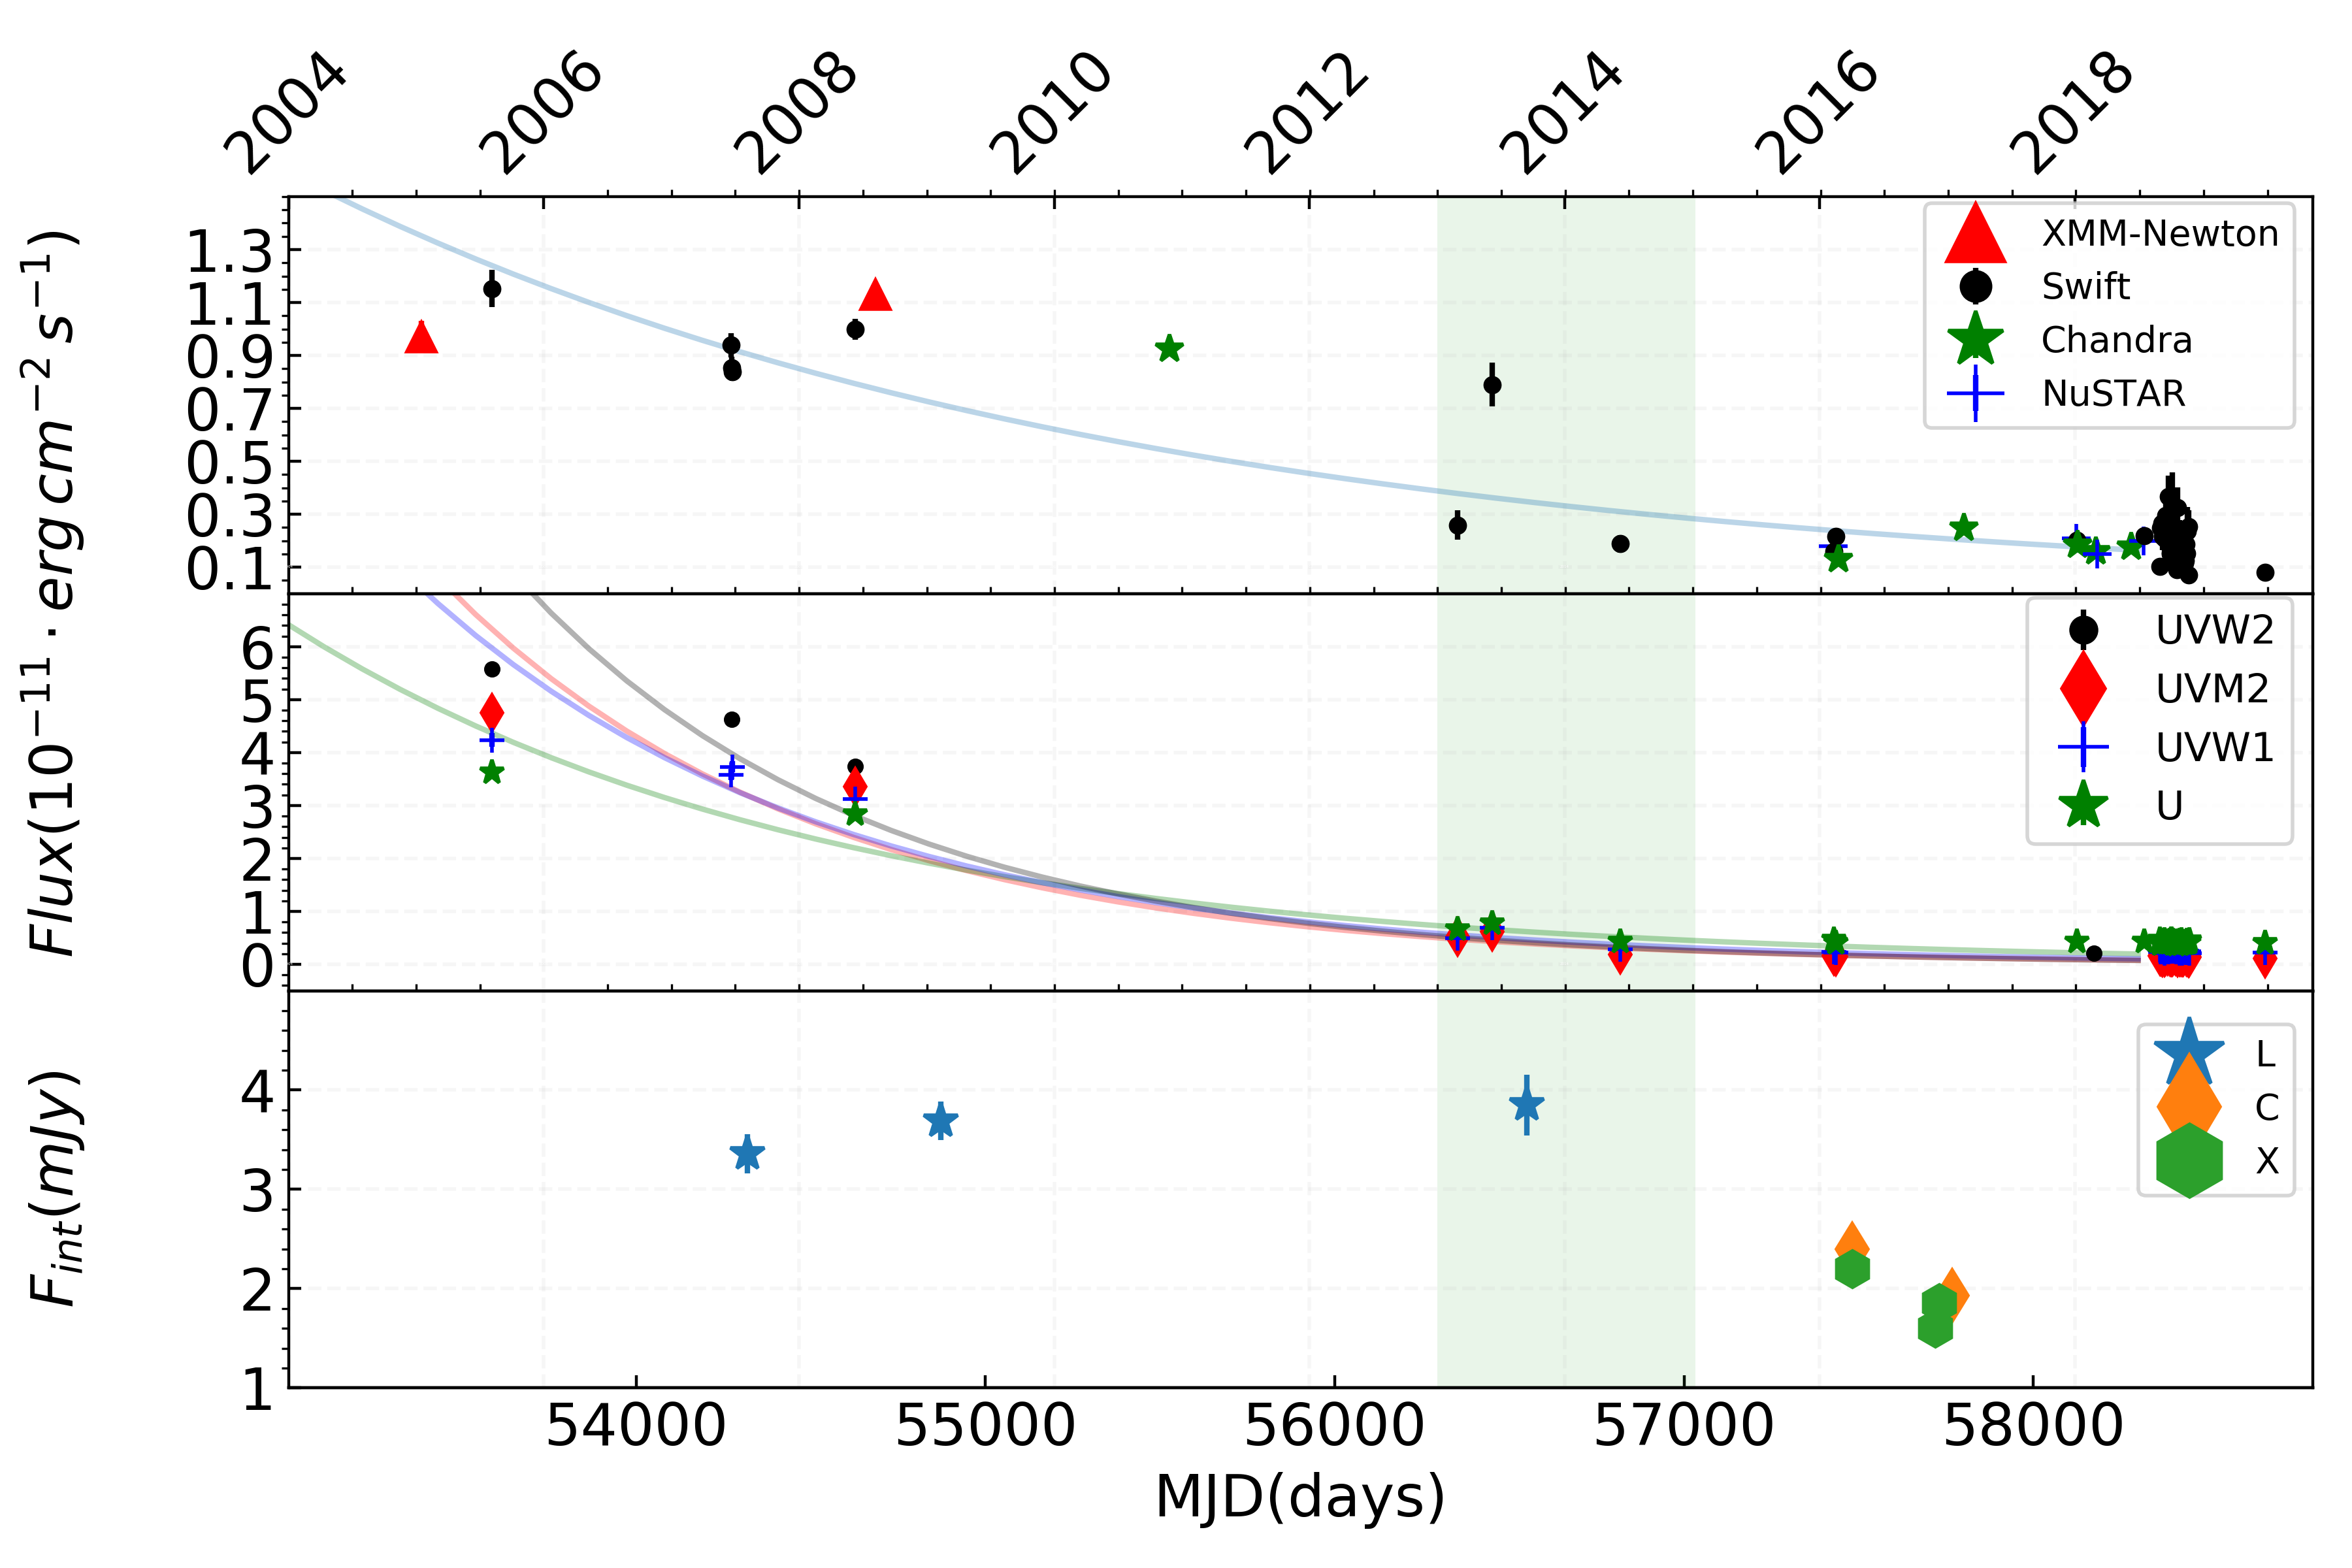
\includegraphics[width=0.9\textwidth]{./pic/subplots-xrt_uvot-radio-second.png}
    \caption{Multi-wavelength light curves of Mrk~1018 between 2005 and 2019. Red and blue vertical dashed lines represent the time of optical spectroscopic confirmation at type 1 and type 1.9, respectively. Region between them is marked as changing-look phase. Grey shallow region shows that the type transition occurred between 2013 and 2015 inferred by \citet{2017A&A...607L...9K} due to the rapid dimming of X-ray flux. Horizontal dotted line in the top panel represents that X-ray flux keeps almost constant until around 2009. The inclined dotted lines in the top and middle panel show the fitting of light curve in X-ray and UV band between 2008 and 2015 with characteristic \textit{e}-folding decay timescale $\tau$. In faint state after 2016, there is rapid variability in X-ray and UV band (see also \autoref{fig:x-ray-uv-lc-rp-secondaxis} for details). At the bottom panel, the label ``$F_\mathrm{5\,GHz}$'' marked with blank circles represent the radio flux scaled to 5 GHz. The whole radio light curve including the period before 2005 is shown in \autoref{fig:radio-lc}.}
    \label{fig:multi-lc-secondaxis}
\end{figure*}


\begin{figure*}
\centering
	% To include a figure from a file named example.*
	% Allowable file formats are eps or ps if compiling using latex
	% or pdf, png, jpg if compiling using pdflatex
	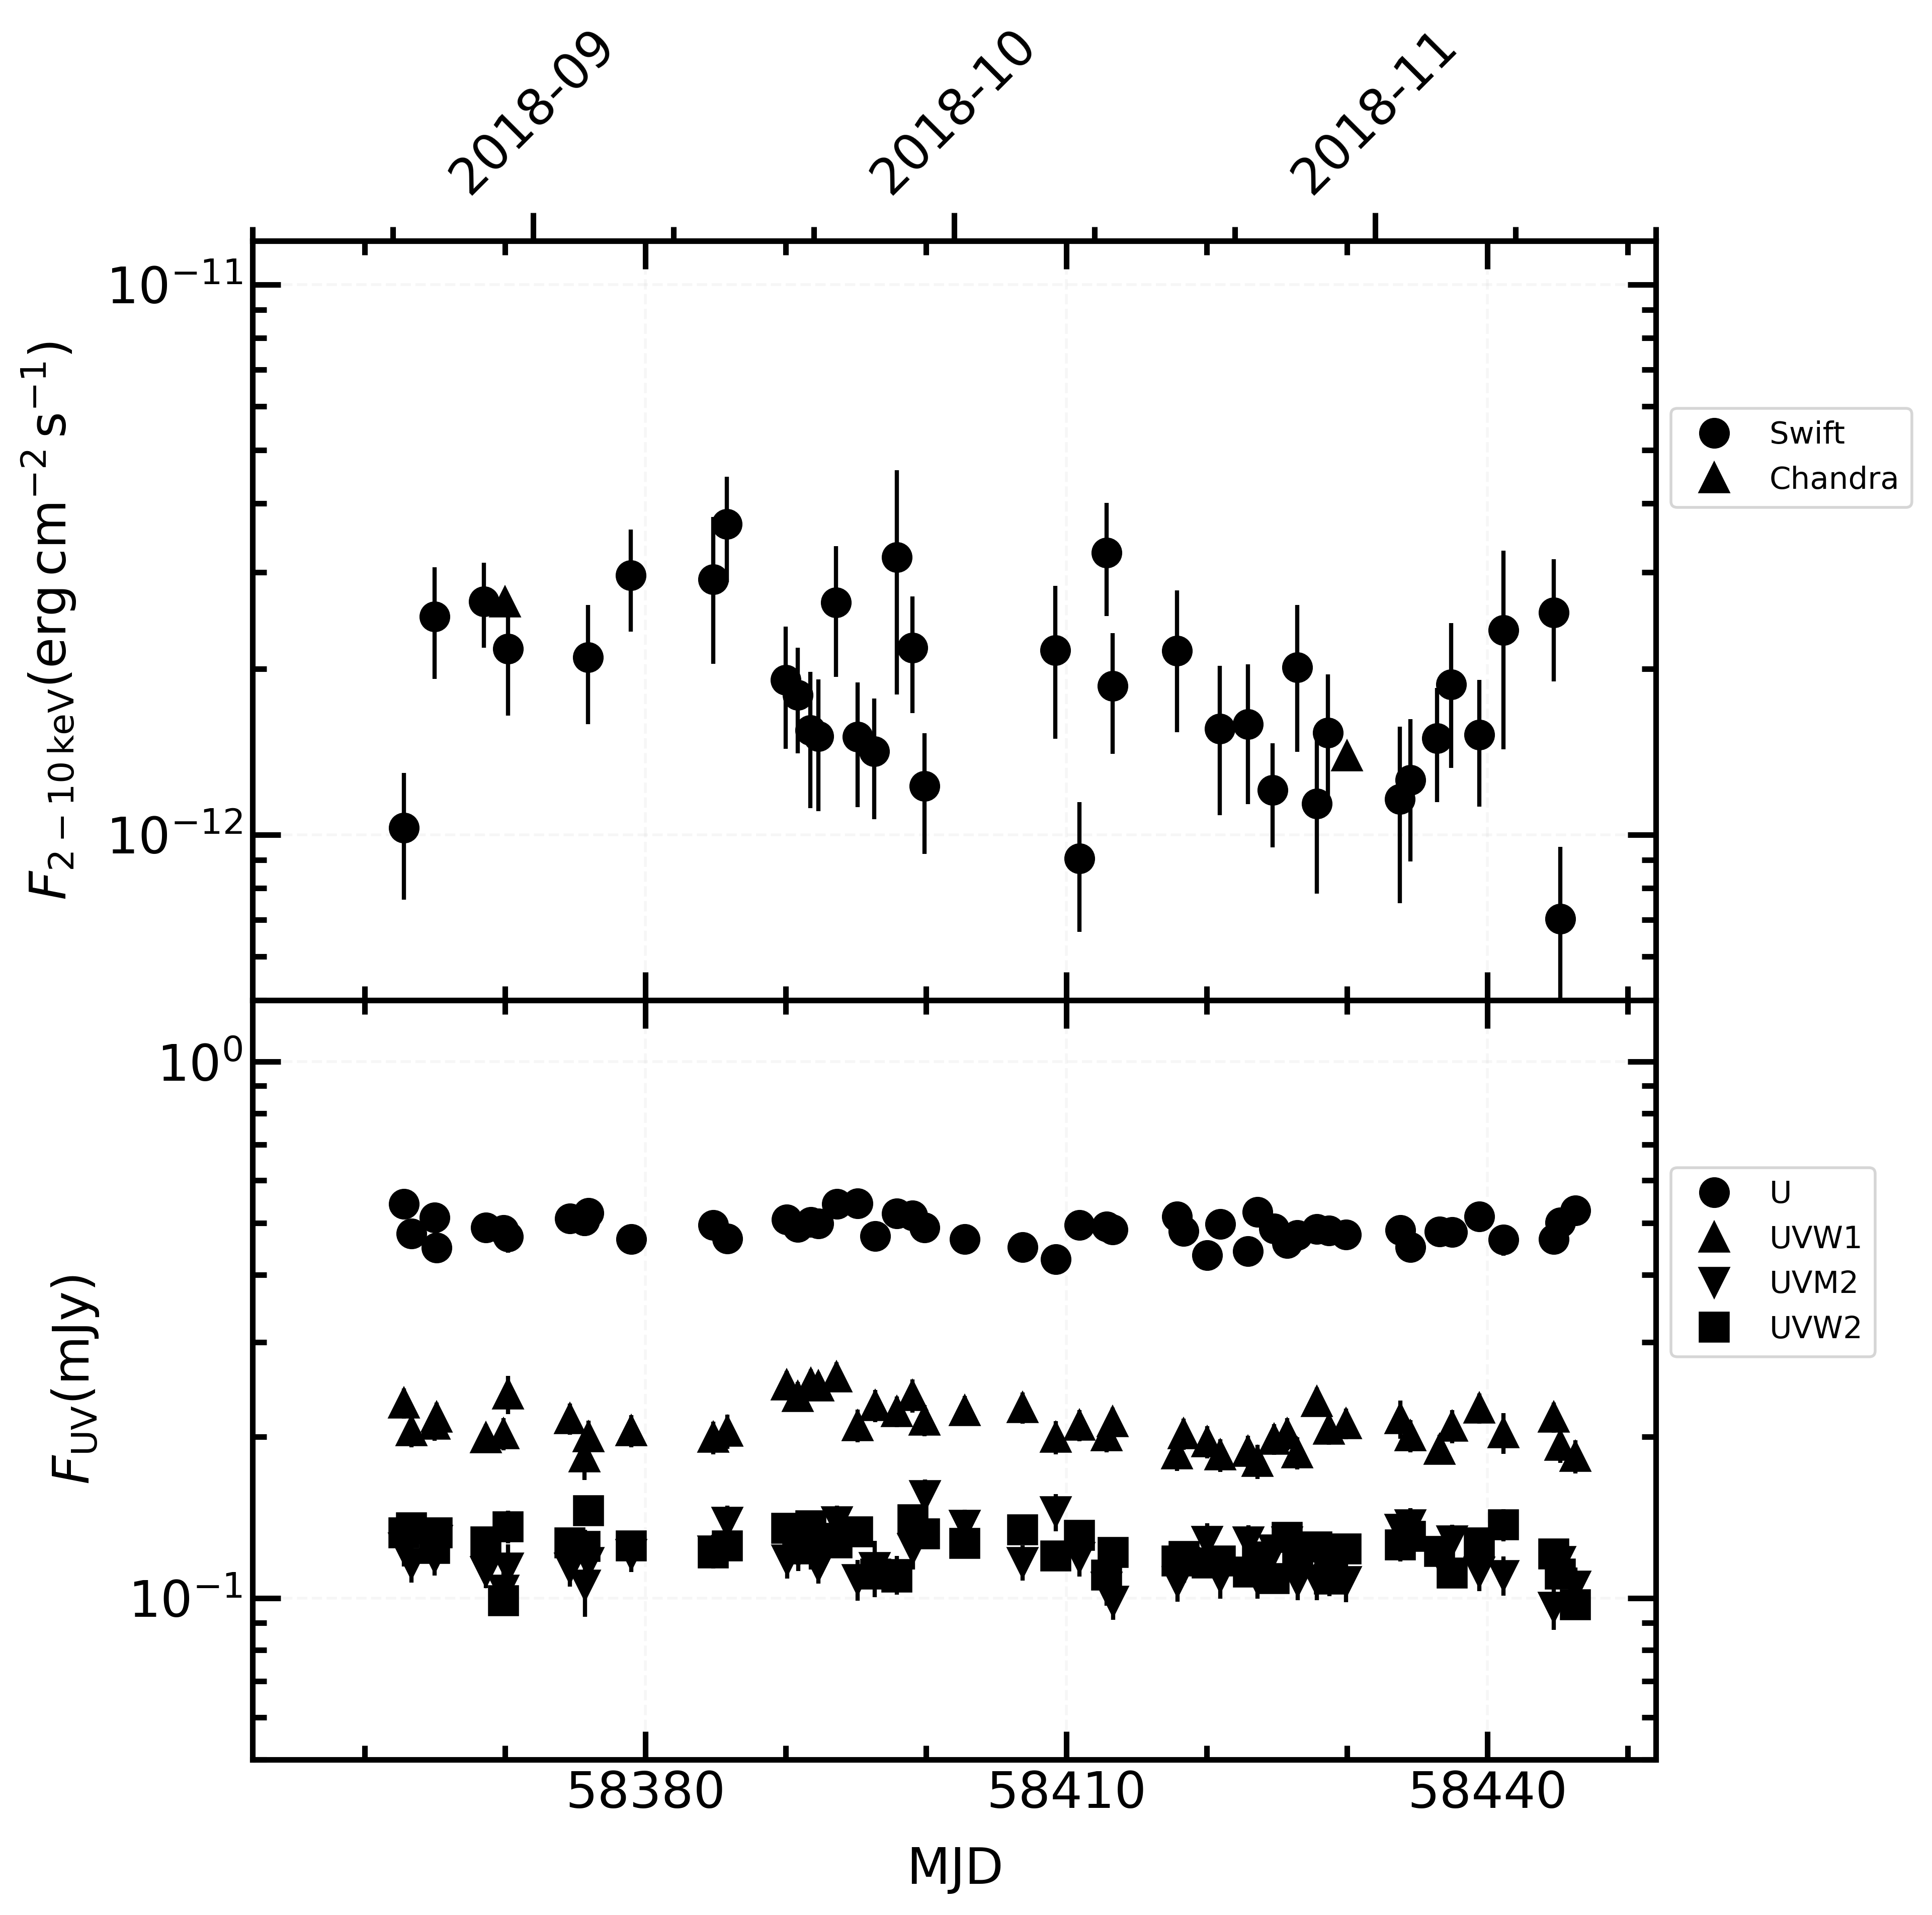
\includegraphics[width=0.9\textwidth]{./pic/subplots-xrt_uvot-radio-second-right-part.png}
    \caption{Light curves of Mrk~1018 in X-ray and UV band with high-cadence monitoring observations between 58350 and 58450 MJD.}
    \label{fig:x-ray-uv-lc-rp-secondaxis}
\end{figure*}

\begin{figure*}
\centering
	% To include a figure from a file named example.*
	% Allowable file formats are eps or ps if compiling using latex
	% or pdf, png, jpg if compiling using pdflatex
	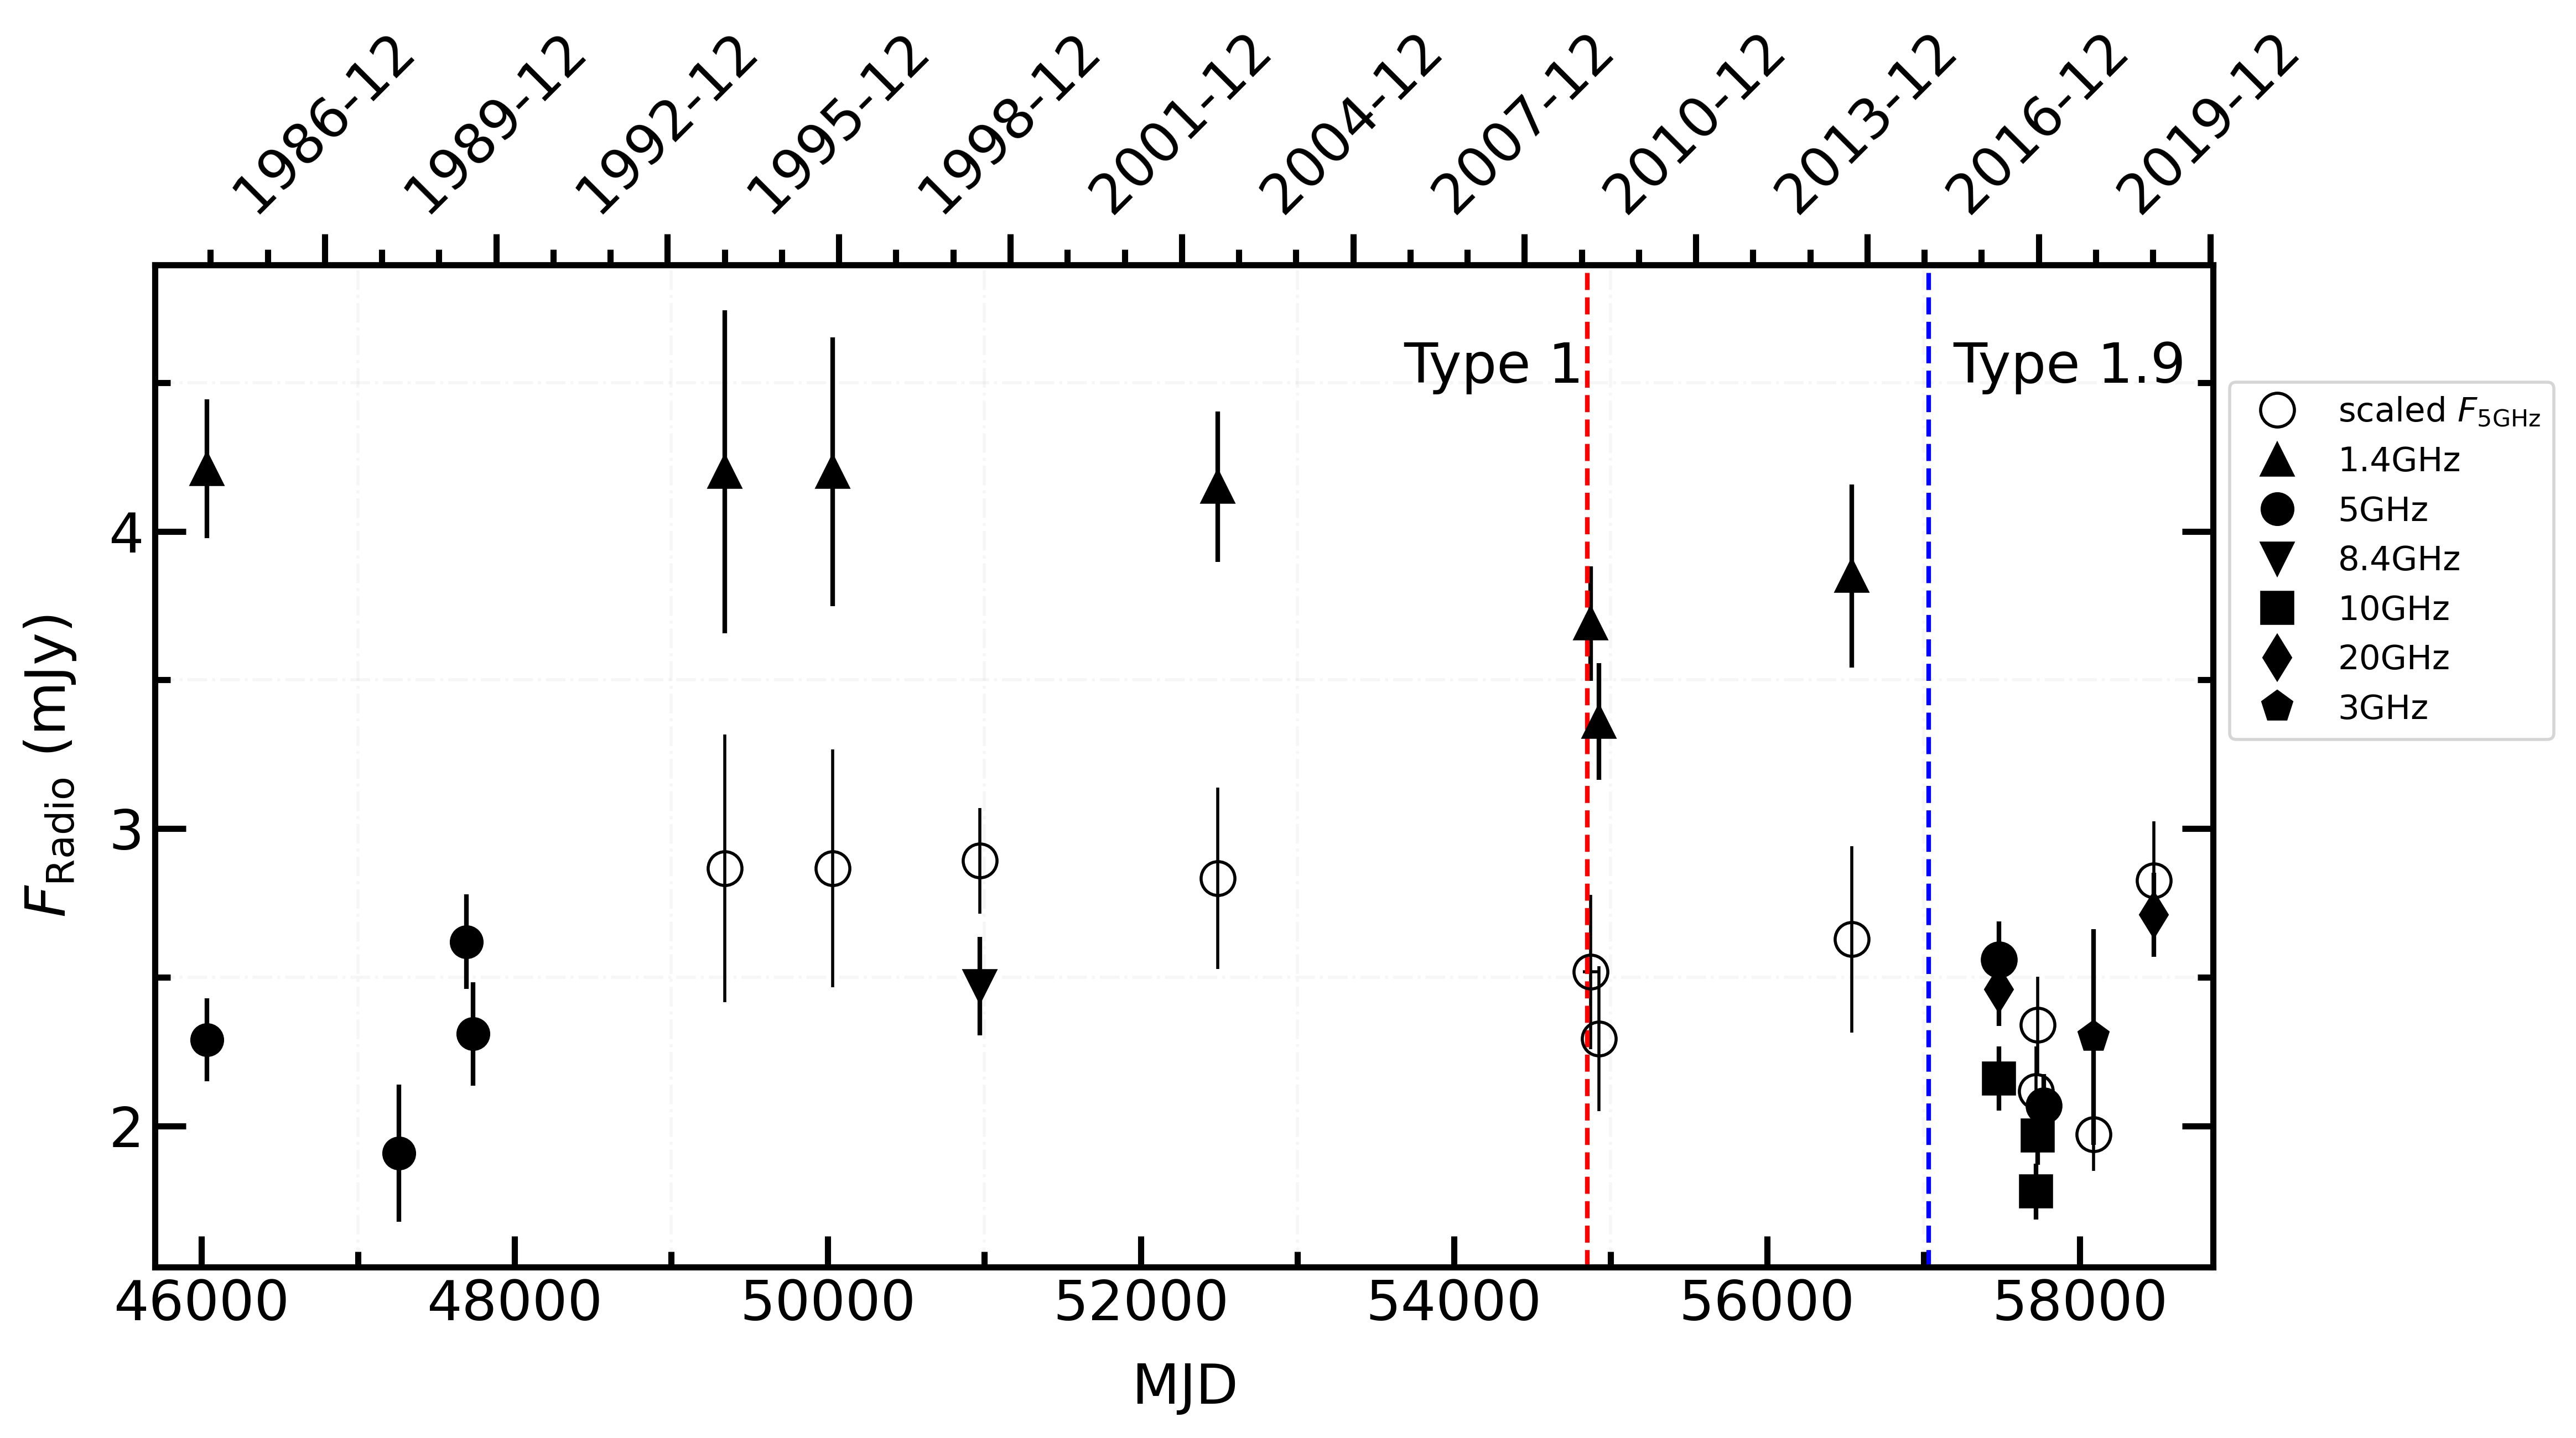
\includegraphics[width=0.9\textwidth]{./pic/subplots-radio-second_freq.png}
    \caption{The radio light curve of Mrk~1018. Filled markers represent the observation flux at corresponding frequency and blank circles represent the radio flux scaled to 5 GHz. Red and blue vertical dashed lines represent the time of optical spectroscopic confirmation at type 1 and type 1.9, respectively.}
    \label{fig:radio-lc}
\end{figure*}




\subsection{Broad-band spectra with \swift\, data}
\label{swift-sed}
Broad-band spectral energy distribution (SED) before and after the changing-look event has been fitted \citep[see][]{2016A&A...593L...9H,2018MNRAS.480.3898N}. As the flux drops in X-ray and UV bands, the broad band SED also changes. On the whole, the shift to left of the peak frequency of UV spectrum is consistent with the decline of disk temperature \citep[also described in][]{2016A&A...593L...9H}. We use the absorbed \texttt{optxagnf} plus S0-type host galaxy emission template named \texttt{hostpol} \citep{2007ApJ...663...81P} model to fit the simultaneous \xrt\, and \uvot \,spectrum. Limited by the data quality, we fix the parameters (electron temperature $kT_e$  and optical depth $\tau$ ) of soft Comptonisation component as same as that estimated in \citet{2018MNRAS.480.3898N}, and photon index $\Gamma$ obtained from the power-law model fitting. We find that bolometric luminosity could be well constrained even though there is large error of determination of coronal radius ($R_\mathrm{cor}$). We fix $f_\mathrm{pl}$, the fraction of the power below $R_\mathrm{cor}$, to 0.85--1.0 \citep[see also][]{2018MNRAS.480.3898N} for observations after 2013 since the luminosity is too low. We get plausible results with $\chi^2_\mathrm{r}$ between 0.68 and 1.23. As the bolometric luminosity declines by around one order of magnitude, the fraction from the contribution of the corona increases from $\sim$ 0.5 to $\sim$0.9, thus the disk luminosity and temperature would also decline considering the less variable $R_\mathrm{cor}$. 

We find a good positive correlation between log($L_\mathrm{X}/L_\mathrm{Edd}$) and log($L_\mathrm{bol}/L_\mathrm{Edd}$), which is parameterised as 
\begin{equation}\label{Lbol-LX}
\log(L_\mathrm{bol}/L_\mathrm{Edd})= 1.52 \times \log( L_\mathrm{X}/L_\mathrm{Edd})+2.25
\end{equation} 
 The Spearman correlation coefficient of two quantities is 0.987 ($p$-value=7.2$\times10^{-7}$). So we use the correlation to derive the bolometric luminosities for other observations without broad-band spectral fitting of \swift\, data. 


\subsection{V-shape $\Gamma$-$L_\mathrm{X}$ correlation and rapid transitions}
The V-shape of $\Gamma$-$L_\mathrm{X}$ correlation, which shows distinct negative/positive correlation with the Eddington scaled X-ray luminosity $L_\mathrm{X}/L_\mathrm{Edd}$ below/above a critical value ($\sim$0.001), has been found in both AGNs and BH XRBs \citep[e.g.][]{2008ApJ...682..212W,2011A&A...530A.149Y,2015MNRAS.447.1692Y}. For Mrk~1018, we also plot the $\Gamma$-$L_\mathrm{X}/L_\mathrm{Edd}$ correlation, which shows evident negative correlation when $L_\mathrm{X}/L_\mathrm{Edd}$ is below the critical value. The positive correlation is less significant when $L_\mathrm{X}/L_\mathrm{Edd}$ is above the critical value since the data are limited. The data of Mrk~1018 roughly follow the two best-fitting lines with $\Gamma$= 1.05$\times$ $\log(L_\mathrm{X}/L_\mathrm{Edd})$ +4.26 and $\Gamma$= -1.15$\times$ $ \log(L_\mathrm{X}/L_\mathrm{Edd})$ -1.98 when the data are divided into right and left branch based on luminosity. The Spearman correlation coefficient between photon index and X-ray luminosity is 0.2 and -0.57 ($p$-values are 0.58 and 4.3$\times10^{-6}$) in right and left branches. We get different slopes of 1.45 and -1.14 at positive and negative branch when fitting with a piecewise linear regression and derive the critical $L_\mathrm{X}/L_\mathrm{Edd}$ value $\sim$ 0.15\%, which corresponds to $L_\mathrm{bol}/L_\mathrm{Edd}\sim$1\% according to \autoref{Lbol-LX}. The best-fitting results in \citet{2015MNRAS.447.1692Y} are also included for comparison (see \autoref{fig:xrayappendgood-Lrateandg-tmap}). For a sample of AGNs, the critical value of $\log(L_\mathrm{X}/L_\mathrm{Edd})$= -3 is close to the individual case of Mrk~1018, but the slopes (0.31 and -0.1) of the positive and the negative branch are much smaller. 

Most of data on the positive branch roughly correspond to the type 1, while data on the negative branch roughly correspond to the type 1.9 assuming that Mrk~1018 is at type 1 before 2009 and at type 1.9 after 2015. However, we find the transitions between two branches during the re-flare (see \autoref{fig:xrayappendgood-Lrateandg-tmap}). The X-ray flux increases by a factor $\sim3$ between 56352 and 56450 MJD, while $\Gamma$ drops from $\sim1.8$ to $\sim1.4$, making it transiting from negative branch to the positive branch, and then returning back to the negative branch on 56817 MJD when the X-ray flux decreases by a factor of $\sim$4.2, and $\Gamma$ does not vary within errors. Unfortunately, the optical spectroscopic type confirmation during the re-flare is absent.


\subsection{Correlation between X-ray and UV luminosity}
\label{subsec:xray-uv}
We use the simultaneous \xrt\, and \uvot\, data between 53587 and 57430 MJD to analyse the relation between X-ray and UV luminosity during the changing-look phase. The 2 keV luminosity $L_\mathrm{{2\,keV}}$ shows a positive correlation with the UV luminosity $L_\mathrm{{UV}}$ during the changing-look phase (see \autoref{fig:correlation-Luvot-L2keV}). We derive the 2 keV flux $F_\mathrm{{2\,keV}}$ from $F_\mathrm{2-10~ keV}$ based on the power-law fitted spectrum.  During the re-flare from 56352 to 56450 MJD, the fluxes in U, UVW1, UVM2 and UVW2 band increase by a factor of 1.16, 1.38, 1.18 and 1.52, which are much smaller than the variability mentioned above in X-ray band, making the re-flare an outlier in the $L_\mathrm{{2\,keV}}$-$L_\mathrm{{UV}}$ correlation. So we exclude the outlier and re-fit the correlation with $\log{L_\mathrm{{2\,keV}}}$=$\gamma$  $\log{L_\mathrm{{UV}}}$+$\beta$, where the slopes $\gamma$ are 1.03, 0.74, 0.66 and 0.63, respectively. The Spearman correlation coefficients between simultaneous luminosity of \xrt\, and four \uvot\, band (U, UVW1, UVM2 and UVW2) are 0.99, 0.93, 0.90 and 0.89 ($p$-values are 1.4$\times10^{-24}$, 2.5$\times10^{-3}$, 0.037 and 0.018), respectively. We do not find evident correlation between X-ray and UV flux during the faint type 1.9 AGN phase.

 




\section{Discussion}\label{sec:discussion}
\subsection{Long and short term variability timescales}
\label{sec:timescale}
We derive three characteristic timescales when Mrk~1018 transited from type 1 to type 1.9 with rapid dimming of luminosity. The \textit{e}-folding decay timescale is $\sim$ 800--1200 days for UV/X-ray band between 2009 and 2015. We find the rise timescale of the re-flare for Mrk~1018 as short as $\sim$98 days. Such re-flares within several tens to hundreds of days are also found in some other CL-AGNs \citep[e.g.][]{2017MNRAS.467.1496O,2020MNRAS.498..718O}. According to the high-cadence monitoring observations, we also find that the X-ray luminosity vary dramatically on timescale of tens of days (see \autoref{fig:x-ray-uv-lc-rp-secondaxis}) when Mrk~1018 is in the faint type 1.9 AGN phase. The rapid variabilities with comparable amplitude are also seen in a sample of AGNs with \swift\, accretion disk reverberation mapping \citep[see][]{2019ApJ...870..123E}. 



The flux variations of AGNs on different timescales and different wavelengths have been studied for a long time \citep[see reviews in ][]{1997ARA&A..35..445U}. A damped random walk (DRW) process provides a good description of AGN variabilities on timescales of days to years \citep[e.g.][]{2010ApJ...721.1014M,2011ApJ...730...52K}, which could be driven by the variations of the magnetic field in the accretion flow \citep{2004MNRAS.348..111K,2006MNRAS.368..379M,2007A&A...466..793J}. \citet{2004MNRAS.348..111K} has demonstrated that the model can produce small flux fluctuations and also stochastic large flares. It seems to be a promising explanation for the long and short variability of CL-AGNs like Mrk~1018. 

\citet{2018MNRAS.480.3898N} has made an analogy between the broad band spectral evolution of Mrk~1018 and the soft-to-hard state transition during the decay phase of transient BHBs. However, the decay timescale is an issue for this analogy, since the decay timescale of an outburst of transient BHB corresponds to the viscous timescale of outer accretion disk. Scaling to a $10^{8}M_{\odot}$ BH, the viscous timescale at typical outer disk radius of $R_\mathrm{disk}$ around hundreds of $R_g$ is roughly one million years \citep{2012MmSAI..83..469L,2018MNRAS.475.1190Y}, which is much longer than characteristic \textit{e}-folding decay timescale we get in Mrk~1018.  

Recently, more and more studies show that the behaviors of CL-AGNs somehow are quite similar to the spectral state transitions in Galactic BH XRBs, and the mechanism caused the spectral state transitions in BH XRBs should also work in the CL-AGNs. However, this will bring an issue about the timescale, which has been noticed by previous works \citep[e.g. ][]{2018NatAs...2..102L,2018ApJ...864...27S,2018MNRAS.480.3898N,2020MNRAS.492.2335L}. The state transtions in BHXRBs normally occur on timescale of days to tens of days \citep{2009ApJ...701.1940Y,2010MNRAS.403...61D}. The state transition timescale is usually
attributed to the viscous timescale of the truncated disk \citep[see reviews in ][]{2007A&ARv..15....1D}, where the viscosity timescale $\tau_\mathrm{vis}$ is given as
\begin{equation}
\tau_\mathrm{vis} \sim 5.7\times 10^{-3} \alpha^{-1}(\frac{M_\mathrm{BH}}{10^8M_{\odot}})(\frac{R_\mathrm{tr}}{R_g})^{3/2} (\frac{H}{R})^{-2} \, \mathrm{days} \end{equation} 
and the disk height is implied as
\begin{equation}
H/R = c_s/v_{\phi}=\frac{\sqrt{kT/m_p}}{\sqrt{GM/R}}
\end{equation} 
where the $c_s$ is the sound speed and $v_{\phi}$ is the Keplarian velocity, and we assume $T\propto R^{-3/4}$. Here we adopt typical value for $T_\mathrm{disk}=3\times10^4\, K$ in a thin disk scenario at R$\sim$100$R_g$ and viscosity coefficient $\alpha=0.1$ \citep[see also][]{2018MNRAS.480.3898N}. Current observations show that the AGN type transition usually occurs on timescale of few years \citep[e.g.][]{2016A&A...593L...8M,2018ApJ...864...27S,2019MNRAS.483L..88P,2020MNRAS.492.2335L} or even few months \citep{2019ApJ...883...94T}. So different models are proposed to produce such short transition timescale, such as a thick disk supported by the magnetic pressure \citep{2019MNRAS.483L..17D}, the radiation pressure instability and  transition between standard disk and optically thin Advection-Dominated
Accretion Flow (ADAF) \citep{2019arXiv190406767S} and the thermal timescale of the disk heating or cooling front \citep{2018ApJ...864...27S}. On the other hand, there are few cases that the state transitions in BH XRBs occur within few hours or even less \citep[e.g.][]{2011A&A...533A...8B,2020A&A...634A..94K} during a highly variable period. The mechanism of this kind of rapid spectral transition is still unknown, which could be a similar mechanism to drive the spectral evolution in CL-AGNs.

\citet{2018ApJ...861...51K} consider the tidal impulse effect within a recoiling-SMBH scenario to explain the long-term variability. The impulse make influence on the density perturbation of accretion disk on the sound crossing timescale $\tau_\mathrm{s}$, which is given as
\begin{equation}
\tau_\mathrm{s} \sim 70 (\frac{M_\mathrm{BH}}{10^8M_{\odot}})(\frac{R_d}{1000 R_g}) (\frac{T}{10^5 K})^{-1/2} \, \mathrm{years}
\end{equation}

While the viscous timescale and the perturbation characterized by the sound crossing timescale are too long compared to the characteristic \textit{e}-folding decay timescale, the thermal timescale could be considered as the origin of the short-term ( tens of days) variability in CL-AGNs. The thermal instability timescale $\tau_\mathrm{th}$ is given as
\begin{equation}
\tau_\mathrm{th} \sim \frac{\tau_\mathrm{dy}}{\alpha} \sim 5.7\times 10^{-3} \alpha^{-1}(\frac{M_\mathrm{BH}}{10^8M_{\odot}})(\frac{R_d}{R_g})^{3/2} \, \mathrm{days}
\end{equation}
Turn-on for CL-AGN could happen at timescale as short as $\sim$70 days\citep[e.g.][]{2019MNRAS.487.4057K},  which is suggested to be mostly compatible with the thermal timescale of $\sim$ 99 days assuming an optical emission distance of R $\sim$ 400 $R_g$. In the case of Mrk~1018, the re-flare rise timescale $\sim$ 98 days is also more consistent with the thermal timescale assuming a suitable emission radius. Coincidently, the transitions between different branches of V-shape $\Gamma$--$L_\mathrm{X}$ correlation happen during the re-flare of Mrk~1018. Besides, it is suggested that timescale of months with 10--20 percent optical variability typically found in AGNs is linked to thermal timescale \citep[see also discussion in ][]{2018MNRAS.480.3898N}. We plot the different timescales as a function of emission radius (R) in \autoref{fig:timescale} as summary. 
\begin{figure*}
\centering
	% To include a figure from a file named example.*
	% Allowable file formats are eps or ps if compiling using latex
	% or pdf, png, jpg if compiling using pdflatex
	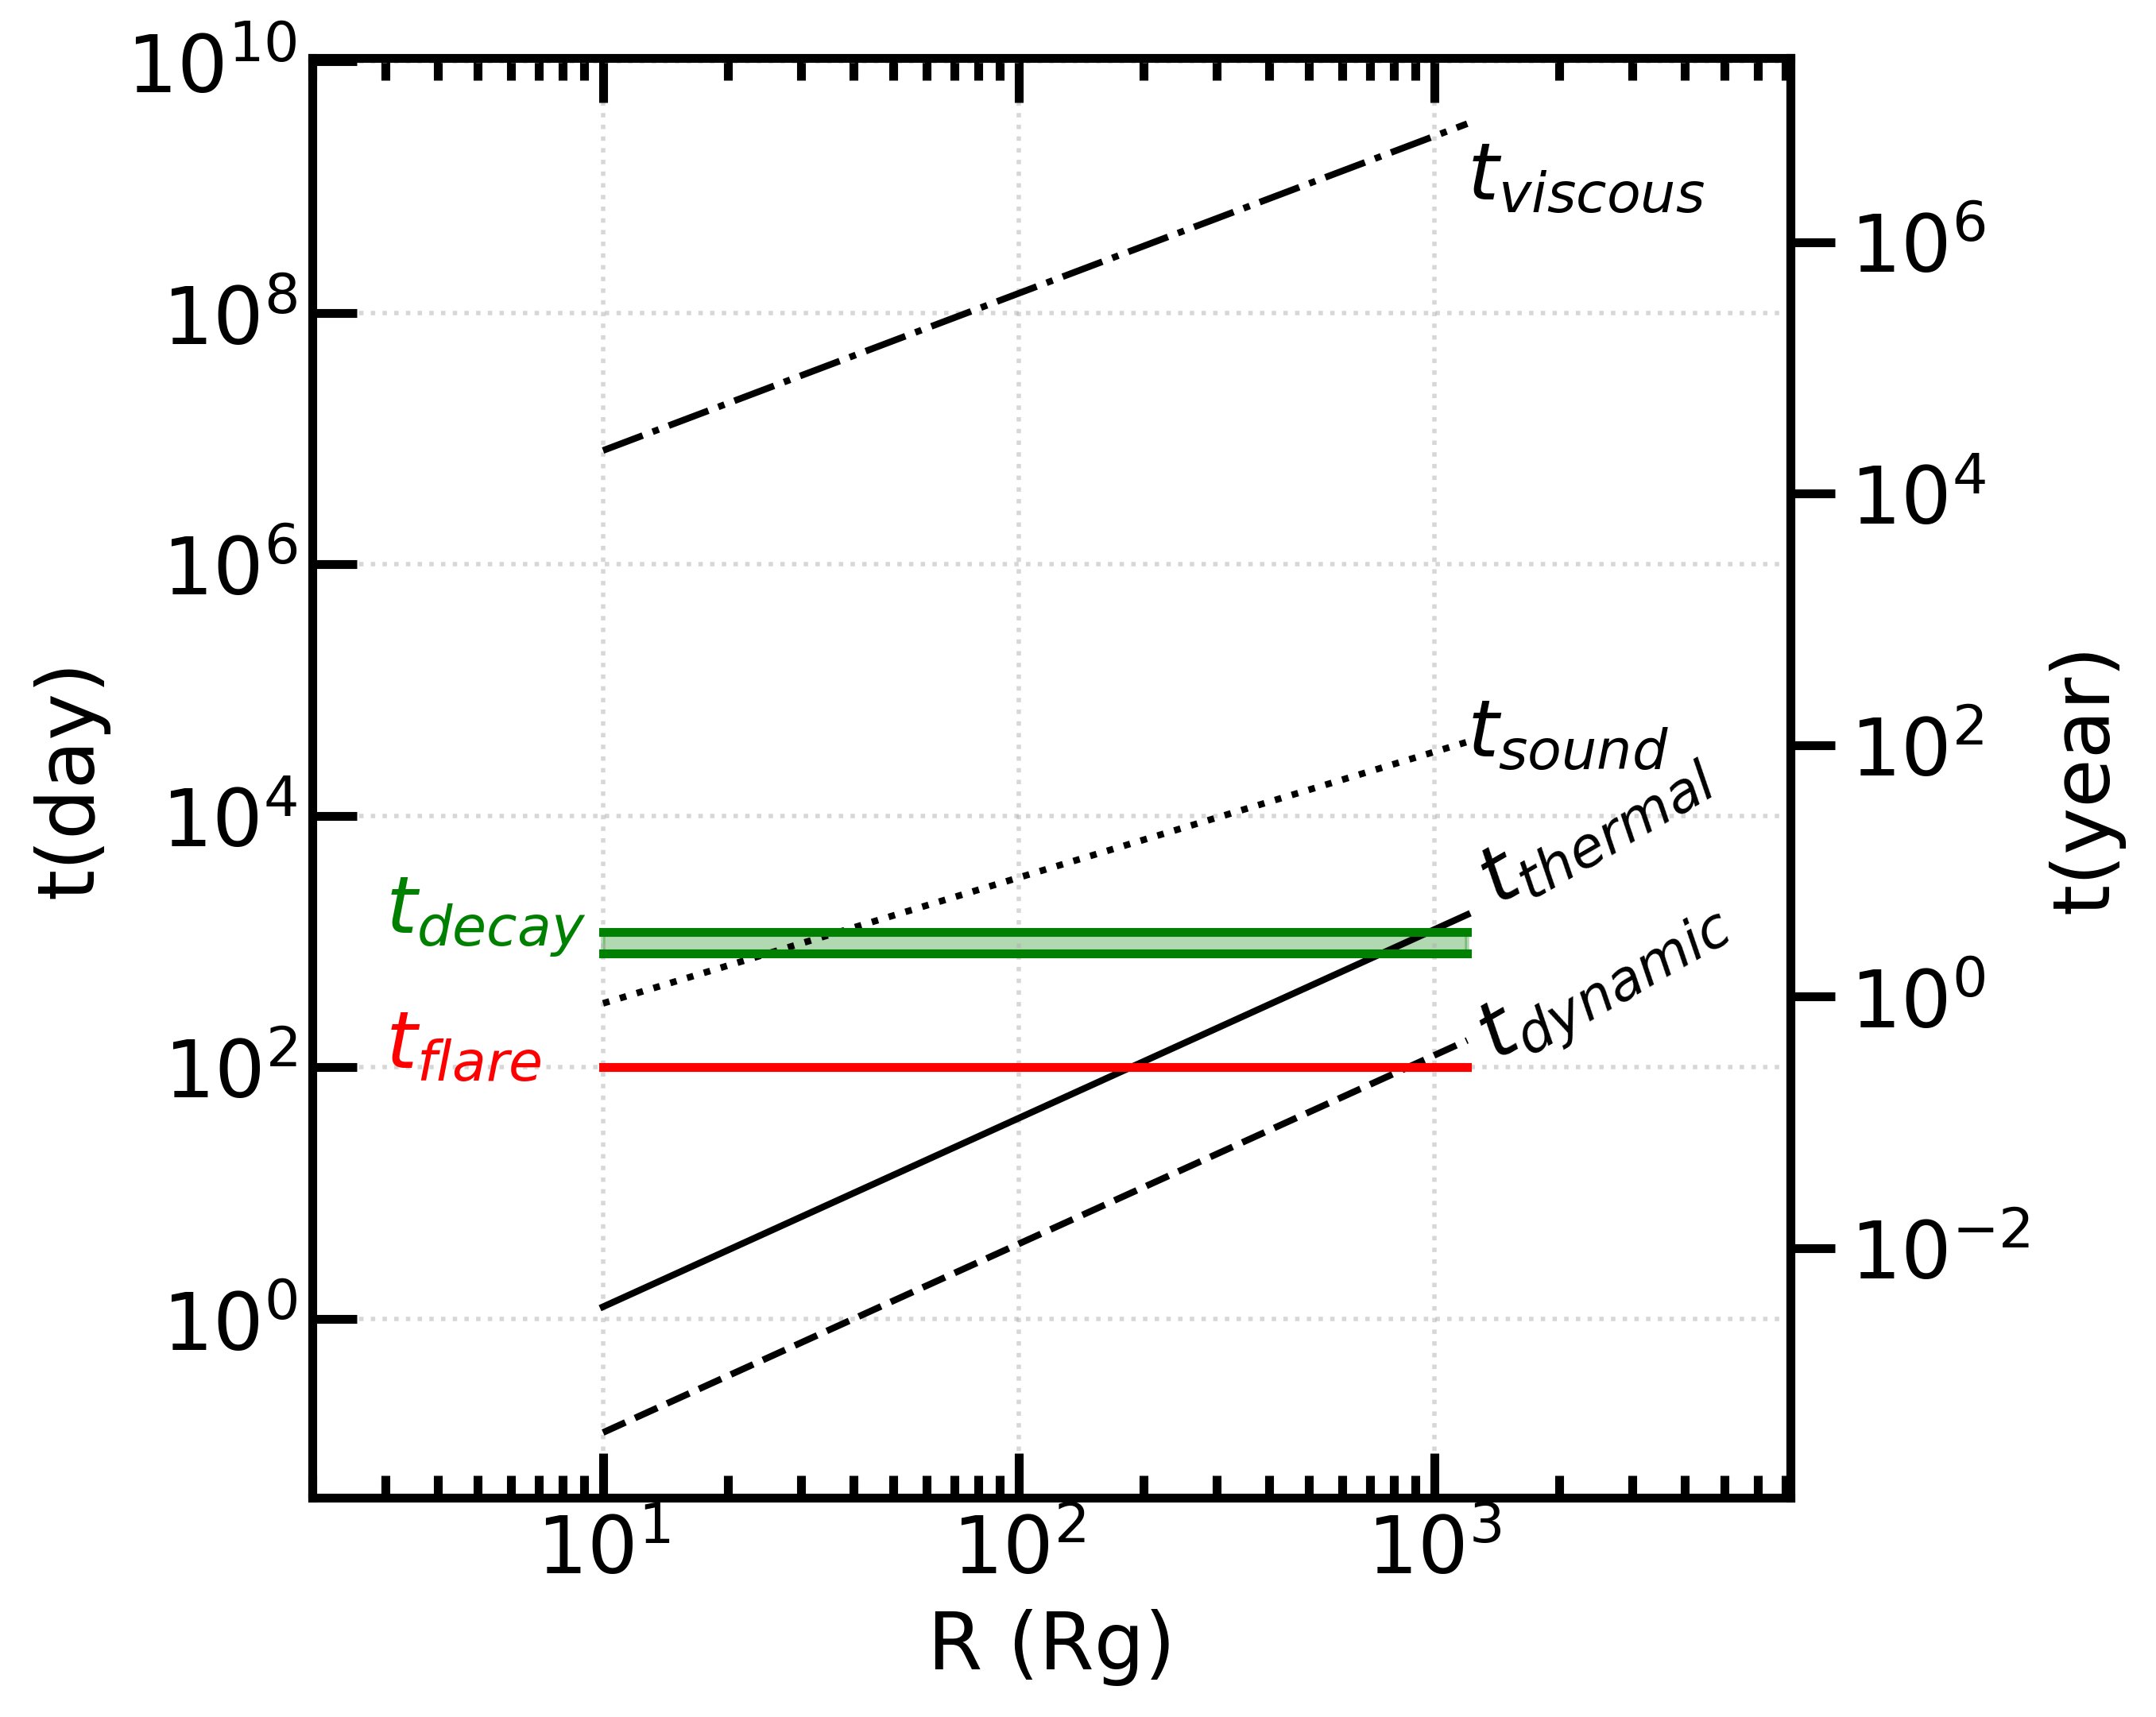
\includegraphics[width=0.8\textwidth]{./pic/Mrk1018_timescale_withR.png}
    \caption{Different timescales as a function of emission radius correspond to the viscosity timescale $t_\mathrm{vis}$, the dynamical timescale $t_\mathrm{dy}$, the thermal timescale $t_\mathrm{th}$ and the sound crossing timescale $t_\mathrm{sound}$. Two horizontal colored lines correspond to the \textit{e}-folding decay timescale $t_\mathrm{decay}$ $\sim$800-1200 days and the re-flare rise timescale $t_\mathrm{flare}$ $\sim$ 98 days, which correspond to the thermal timescale at $\sim$1000 and $\sim$ 200 $R_g$, respectively.}
    \label{fig:timescale}
\end{figure*}


\subsection{Accretion mode changes}
\label{sec:spectral evolution}

 The case of Mrk~1018 that demonstrates the V-shape $\Gamma$-$L_\mathrm{X}$ correlation holds in individual source \citep[see also in ][etc]{2020ApJ...890L..29A}. Similar phenomenon has also been observed in the normal AGNs (relative to CL-AGNs) over a large luminosity range \citep[e.g. ][]{2009MNRAS.399..349G, 2011A&A...530A.149Y}. It is interesting to note that the pivoting points of the V-shape correlations of CL-AGNs and normal AGNs show almost the same value of $L_\mathrm{X}/L_\mathrm{Edd}\sim 10^{-3}$. It is well known that the X-ray emission of an AGN is from the Compton scattering in the hot corona \citep[e.g.][]{1991ApJ...380L..51H}. In the normal AGNs, the reason for the opposite X-ray spectral behavior is thought to be the differences of the seed photons for the Compton scattering, i.e. the seed photons are from the synchrotron emission of the hot corona itself at the lower luminosity branch, while from the thermal emission from Shakura–Sunyaev disk \citep[SSD; e.g. ][]{2013ApJ...764....2Q} or other thermal component \citep{2015MNRAS.447.1692Y} at the higher luminosity branch. So the same mechanism should also work in Mrk 1018, i.e. an extra thermal component (such as SSD) which provides the external seed photons appears/disappears above/below the critical luminosity in addition to the hot corona. Mrk~1018's approximate V-shape $\Gamma$--$L_\mathrm{X}$ correlation supports the idea that the accretion mode changes. The accretion mode changes have also been suggested in other CL-AGNs or highly variable AGN \citep{2019arXiv191203972L,2020ApJ...890L..29A,2020MNRAS.492.2335L}.  If the AGN type transitions indeed associates with the accretion mode changes, the AGNs at the luminosity level of $L_\mathrm{bol}/L_\mathrm{Edd}\sim 10^{-2}$ would be the candidates of changing-look AGNs, since the stochastic variation (see discussion in \autoref{sec:timescale}) can easily make the luminosity above/below the critical luminosity to change the accretion mode. 
 
It has been observed that the broad line luminosity is positively correlated with the UV luminosity, and the broad line width is negatively correlated with the UV luminosity \citep[e.g.][]{2019ApJ...885...44D}. In the case of Mrk~1018, if the inner disk disappears at the low luminosity, which is consistent with the decreasing of the disk temperature \citep[see also ][]{2018MNRAS.480.3898N}, the decreased UV luminosity will cause the weaker and broadened line component non-detected. On the other hand, some models of the broad line region are indeed related with the SSD, which can be account for the type transition in the CL-AGNs \citep[see a recent review in ][and references therein]{2019OAst...28..200C}. For example, in the disk-wind model of the BLR origin, the AGNs evolve from type 1 to type 1.9 as the luminosity decreases \citep[see][]{2014MNRAS.438.3340E}. \citet{2018MNRAS.480.3898N} suggests that the soft X-ray excess contributes most ionizing photons, and the drop of soft X-ray excess causes the disappearance of broad emission line \citep[see also in ][]{2020MNRAS.492.2335L}. However, the origin of the soft excess is still under debate \citep[e.g.][]{2018A&A...611A..59P}.  

The optical/UV-to-X-ray spectral index \alphaox\, is also a good indicator of the broad SED, which has been used extensively for a long time \citep[e.g.][]{1979ApJ...234L...9T}. Here we define \alphaox\, as 
%\begin{equation}
%\alpha_{OX}  = - \frac{\log(\lambda F_{2600 \angstrom}/\nu F_{2keV})}{\log(\nu_{ 2600 \angstrom }/\nu_{2keV})}+1
%\end{equation}
\begin{equation}
\alpha_\mathrm{OX} = \frac{\log (L_\mathrm{UV} / L_\mathrm{2keV} )} {\log (\nu_\mathrm{2keV} /  \nu_\mathrm{UV} )}=\frac{\log (L_\mathrm{UV} / L_\mathrm{2keV} )}{2.623}
\label{definition_alpha_ox}
\end{equation}
, where the $L_\mathrm{UV}$ is from the UVW1 filter with central wavelength {2600{$\angstrom$}} and full-width at half max of $\sim 683\angstrom$ \citep{2008MNRAS.383..627P} and the $L_\mathrm{2keV}$ is the 2 keV luminosity.



It is also found that  \alphaox\, is positively correlated with the luminosity in different luminous AGNs samples \citep[e.g.][]{2010A&A...512A..34L, 2013A&A...550A..71V,2016ApJ...819..154L}, and negatively correlated with the luminosity in the low luminosity AGNs \citep[e.g.][]{2011ApJ...739...64X,2017MNRAS.471.2848L}. The dividing line of these two opposite correlations is roughly at $L_\mathrm{bol}/L_\mathrm{Edd} \sim$ $10^{-3}$ \citep{2011ApJ...739...64X,2017MNRAS.471.2848L}. The hot accretion flow is thought to dominate the broad band emission from optical to X-ray in the LLAGNs \citep[see reviews in ][]{2014ARA&A..52..529Y}. While the X-ray is from Compton scattering of the hot corona, and the optical/UV emission originates from the SSD in the luminous AGNs. At the same time, the hot accretion flow can roughly explain the negative \alphaox\,--$L_\mathrm{bol}$ correlation at the lower luminosity branch \citep{2011ApJ...739...64X,2017MNRAS.471.2848L}, and the disk-corona can explain the positive correlation at the higher luminosity branch \citep{2017A&A...602A..79L, 2018MNRAS.480.1247K,2019A&A...628A.135A}. The different relations between \alphaox\, and $L_\mathrm{bol}$ also support the idea that the accretion mode changes in the high and low luminosity AGNs \citep[see][]{2011MNRAS.413.2259S,2019ApJ...883...76R}. 

\citet{2011MNRAS.413.2259S} simulated the spectral states of AGNs by analogy with BHXRBs, and found that the simulated AGNs at different spectral states and luminosities roughly follow a V-shape \alphaox--$L_\mathrm{bol}$ correlation \citep[see also in ][]{2019ApJ...883...76R}. \citet{2019arXiv190904676R} recently finds that two CL-AGNs follow a roughly V-shape \alphaox--$L_\mathrm{UV}$ correlation, although they applied an X-ray reprocessing model to explain the correlation. We also plot the \alphaox\,-$L_\mathrm{X}$ correlation by using their data. It seems that they follow two negative correlations with different slopes for type 1 and type 2 AGNs. The shapes of the \alphaox-$L_\mathrm{X}$ and \alphaox-$L_\mathrm{UV}$ correlations are apparently different. The pivoting luminosity differs from \citet{2011ApJ...739...64X} by almost one order of magnitude. So here is an issue about the bolometric correction of $L_\mathrm{X}$ or $L_\mathrm{UV}$ with a large dynamic range of \alphaox \,and luminosity. Interestingly, Mrk~1018's position in the \alphaox-$L_\mathrm{UV}/L_\mathrm{Edd}$ and \alphaox-$L_\mathrm{X}/L_\mathrm{Edd}$ correlations is well in agreement with type 1 and type 2 branches when we add the data of Mrk~1018 onto the plots of the two CL-AGNs in \citet{2019arXiv190904676R} (see \autoref{fig:alpha_ox_lx_luv}).

However, we find that there is evident positive correlation between $L_\mathrm{2\,keV}$ and $L_\mathrm{UV}$ of Mrk~1018 during the changing-look phase. Before 2016, \alphaox-$L_\mathrm{UV}$ and \alphaox-$L_\mathrm{X}$ correlations are shown in \autoref{fig:alpha_ox_lx_luv}. According to \autoref{definition_alpha_ox}, we derive its byproducts \alphaox $\propto (\frac{1}{\gamma}-1) \log L_\mathrm{2\,keV}$, and \alphaox $\propto (1-\gamma) \log L_\mathrm{UV}$. With $\gamma$ =0.745 (see \autoref{subsec:xray-uv}), \alphaox\, should be linearly correlated with $\log L_\mathrm{X}$ and $\log L_\mathrm{UV}$ with slopes of 0.34 and 0.26, respectively. So the data of Mrk~1018 alone do not show two branches, which need more samples for further investigation. 




%\textcolor{red}{}



\subsection{Relatively flat R-X correlation}
There is a common non-linear correlation between the radio and X-ray luminosity (R-X correlation hereafter) spanning over different mass black holes from the super-massive black holes to stellar mass black holes, where the $L_\mathrm{R}$ is proportional to $L_\mathrm{X}^{0.6}$ \citep{2003MNRAS.345.1057M,2004A&A...414..895F}. However, there are some sources following a steeper R-X correlation with a power-law index of $\sim$1.4 at high $L_\mathrm{X}$, a flat R-X correlation with a power-law index of  $\sim$0 at moderate $L_\mathrm{X}$, and the standard R-X correlation with a powerlaw index $\sim$0.6 at low luminosity \cite[e.g.][]{2011MNRAS.414..677C,2014ApJ...788...52C,2016MNRAS.463.2287X}. The physics of this ``hybrid" R-X correlation is still under debate. The slope change of the correlation may attribute to the different accretion modes or jet physics at low and high luminosity\citep{2016MNRAS.456.4377X,2018MNRAS.481.4513I,2018MNRAS.473.4122E}. 

The 5 GHz radio luminosity and the 2--10 keV X-ray luminosity were used to investigate the R-X correlation. We find that the radio luminosity at 5 GHz only varies within $\sim$40\%, while the X-ray luminosity varies roughly one order of magnitude during the same time interval from 53587 to 58430 MJD (see \autoref{fig:multi-lc-secondaxis}). The radio image shows no distinct extended structure within source size 1.21$''$ $\times$ 0.77 $''$ when Mrk~1018 is observed at the most extensive A configuration of VLA, which corresponds to $\sim$1 kpc-scale region. This might explain why the variability in radio band is lower than X-ray band since the radio emission could originate from larger regions. 

We plot the correlation between the 5 GHz radio luminosity and the nearest X-ray luminosity (interval $\le$ 100 days, see \autoref{tab:radio_xray}) in \autoref{fig:radio-xray-mass_relation_Plotkin2012} and the best-fitting result of a sample of black holes with flat/inverted radio spectra index (e.g. $\alpha_R <$ 0.5) and sub-Eddington luminosity in \citet{2012MNRAS.419..267P}. Our current data show that Mrk 1018 apparently does not follow the standard $L_\mathrm{R}\propto L_\mathrm{X}^{0.6}$ correlation. It roughly follows a flat R-X correlation at the range of $L_\mathrm{X}/L_\mathrm{Edd}$ $\sim$ 3$\times 10^{-4}$-- 4$\times 10^{-3}$ , which is similar to the flat part ($L_\mathrm{bol}/L_\mathrm{Edd} \sim$ $10^{-3}$-$10^{-2}$) of the ``hybrid" correlation in BH XRBs \citep[see e.g.][]{2018MNRAS.473.4122E,2020ApJ...891...31X}. We also superimpose the data of Mrk~590 from \citet[][]{2016MNRAS.460..304K} in \autoref{fig:radio-xray-mass_relation_Plotkin2012} since they share many similarities as CL-AGNs. Both of them show type change from type 1 to type 1.9/2 within years. The ratio of radio and X-ray luminosity $\log(L_R/L_X)$ is $\sim$ -5 to -4 for Mrk~1018 and Mrk~590. Two sources both show the tendency to be flatter of the radio spectrum index ($\alpha_R$) and several tens percent of decline in radio flux as the X-ray luminosity declines by around an order of magnitude. It has been shown that type 2 AGNs roughly have more flat radio spectra, and type 1 AGNs are statistically steeper than type 2 AGNs in some samples\citep[e.g.][]{2019MNRAS.485.3185C}, which is consistent with the CL-AGNs Mrk 1018 and Mrk 590.  More samples are needed to study the systematic radio properties of the CL-AGNs and different types of AGNs.






\section{Summary}
\label{sec:conclusion}
The main observational results of Mrk~1018 are summarized as follows,
\begin{enumerate}
\item We find a re-flare with a rise timescale $\sim 98$ days during the rapid X-ray and UV flux decay in the changing-look phase (\autoref{fig:multi-lc-secondaxis}).

\item $\Gamma$-$L_\mathrm{X}/L_\mathrm{Edd}$ follows a V-shape correlation, where Mrk~1018 shows transitions between the two branches of the V-shape during the re-flare (\autoref{fig:xrayappendgood-Lrateandg-tmap}).

\item  \alphaox-$\nu L_{\nu(\mathrm{2500 \AA})}/L_\mathrm{Edd}$ and \alphaox-$\nu L_{\nu(\mathrm{2\,keV})}/L_\mathrm{Edd}$ correlations are roughly consistent with the type 1 and type 2 branches (\autoref{fig:alpha_ox_lx_luv}) of two CL-AGNs \citep[see][]{2019arXiv190904676R}.

\item Mrk~1018 follows a relatively flat R-X correlation (\autoref{fig:radio-xray-mass_relation_Plotkin2012}). 

\end{enumerate}
Further simultaneous observations in multi-wavelength bands are required to understand the relation between AGN type and spectral state indicated by the V-shape X-ray spectral evolution and the \alphaox-${L_\mathrm{}}$ correlation. 



\acknowledgments
\vspace{5mm}

We thank Chris Done for her friendly help with the usage of host galaxy model, Prof Minfeng Gu for the discussions on the radio observations of CL-AGNs and Dr Linhui Wu and Minhua Zhou for discussions on the VLA data reduction. B.L. and Q.W. are supported in part by the NSFC (grant U1931203); Z.Y. is supported in part by the Natural Science Foundation of China (grants 11773055, U1938114), the Youth Innovation Promotion Association of CAS (ids. 2020265); W.Y. would like to acknowledge the support in part by the National Program on Key Research and Development Project (Grant No.2016YFA0400804) and the National Natural Science Foundation of China (grant number 11333005 and U1838203).

\facilities{\chandra, \xrt, \uvot, \xmm, \nustar, \vla}
%% Similar to \facility{}, there is the optional \software command to allow 
%% authors a place to specify which programs were used during the creation of 
%% the manusscript. Authors should list each code and include either a
%% citation or url to the code inside ()s when available.

\software{HEASOFT(v6.26),
          SAS (v16.1.0),
          CIAO (v4.10), CASA(v5.3.0),
          Astropy
          }
%%

\begin{figure*}
\centering
	% To include a figure from a file named example.*
	% Allowable file formats are eps or ps if compiling using latex
	% or pdf, png, jpg if compiling using pdflatex
	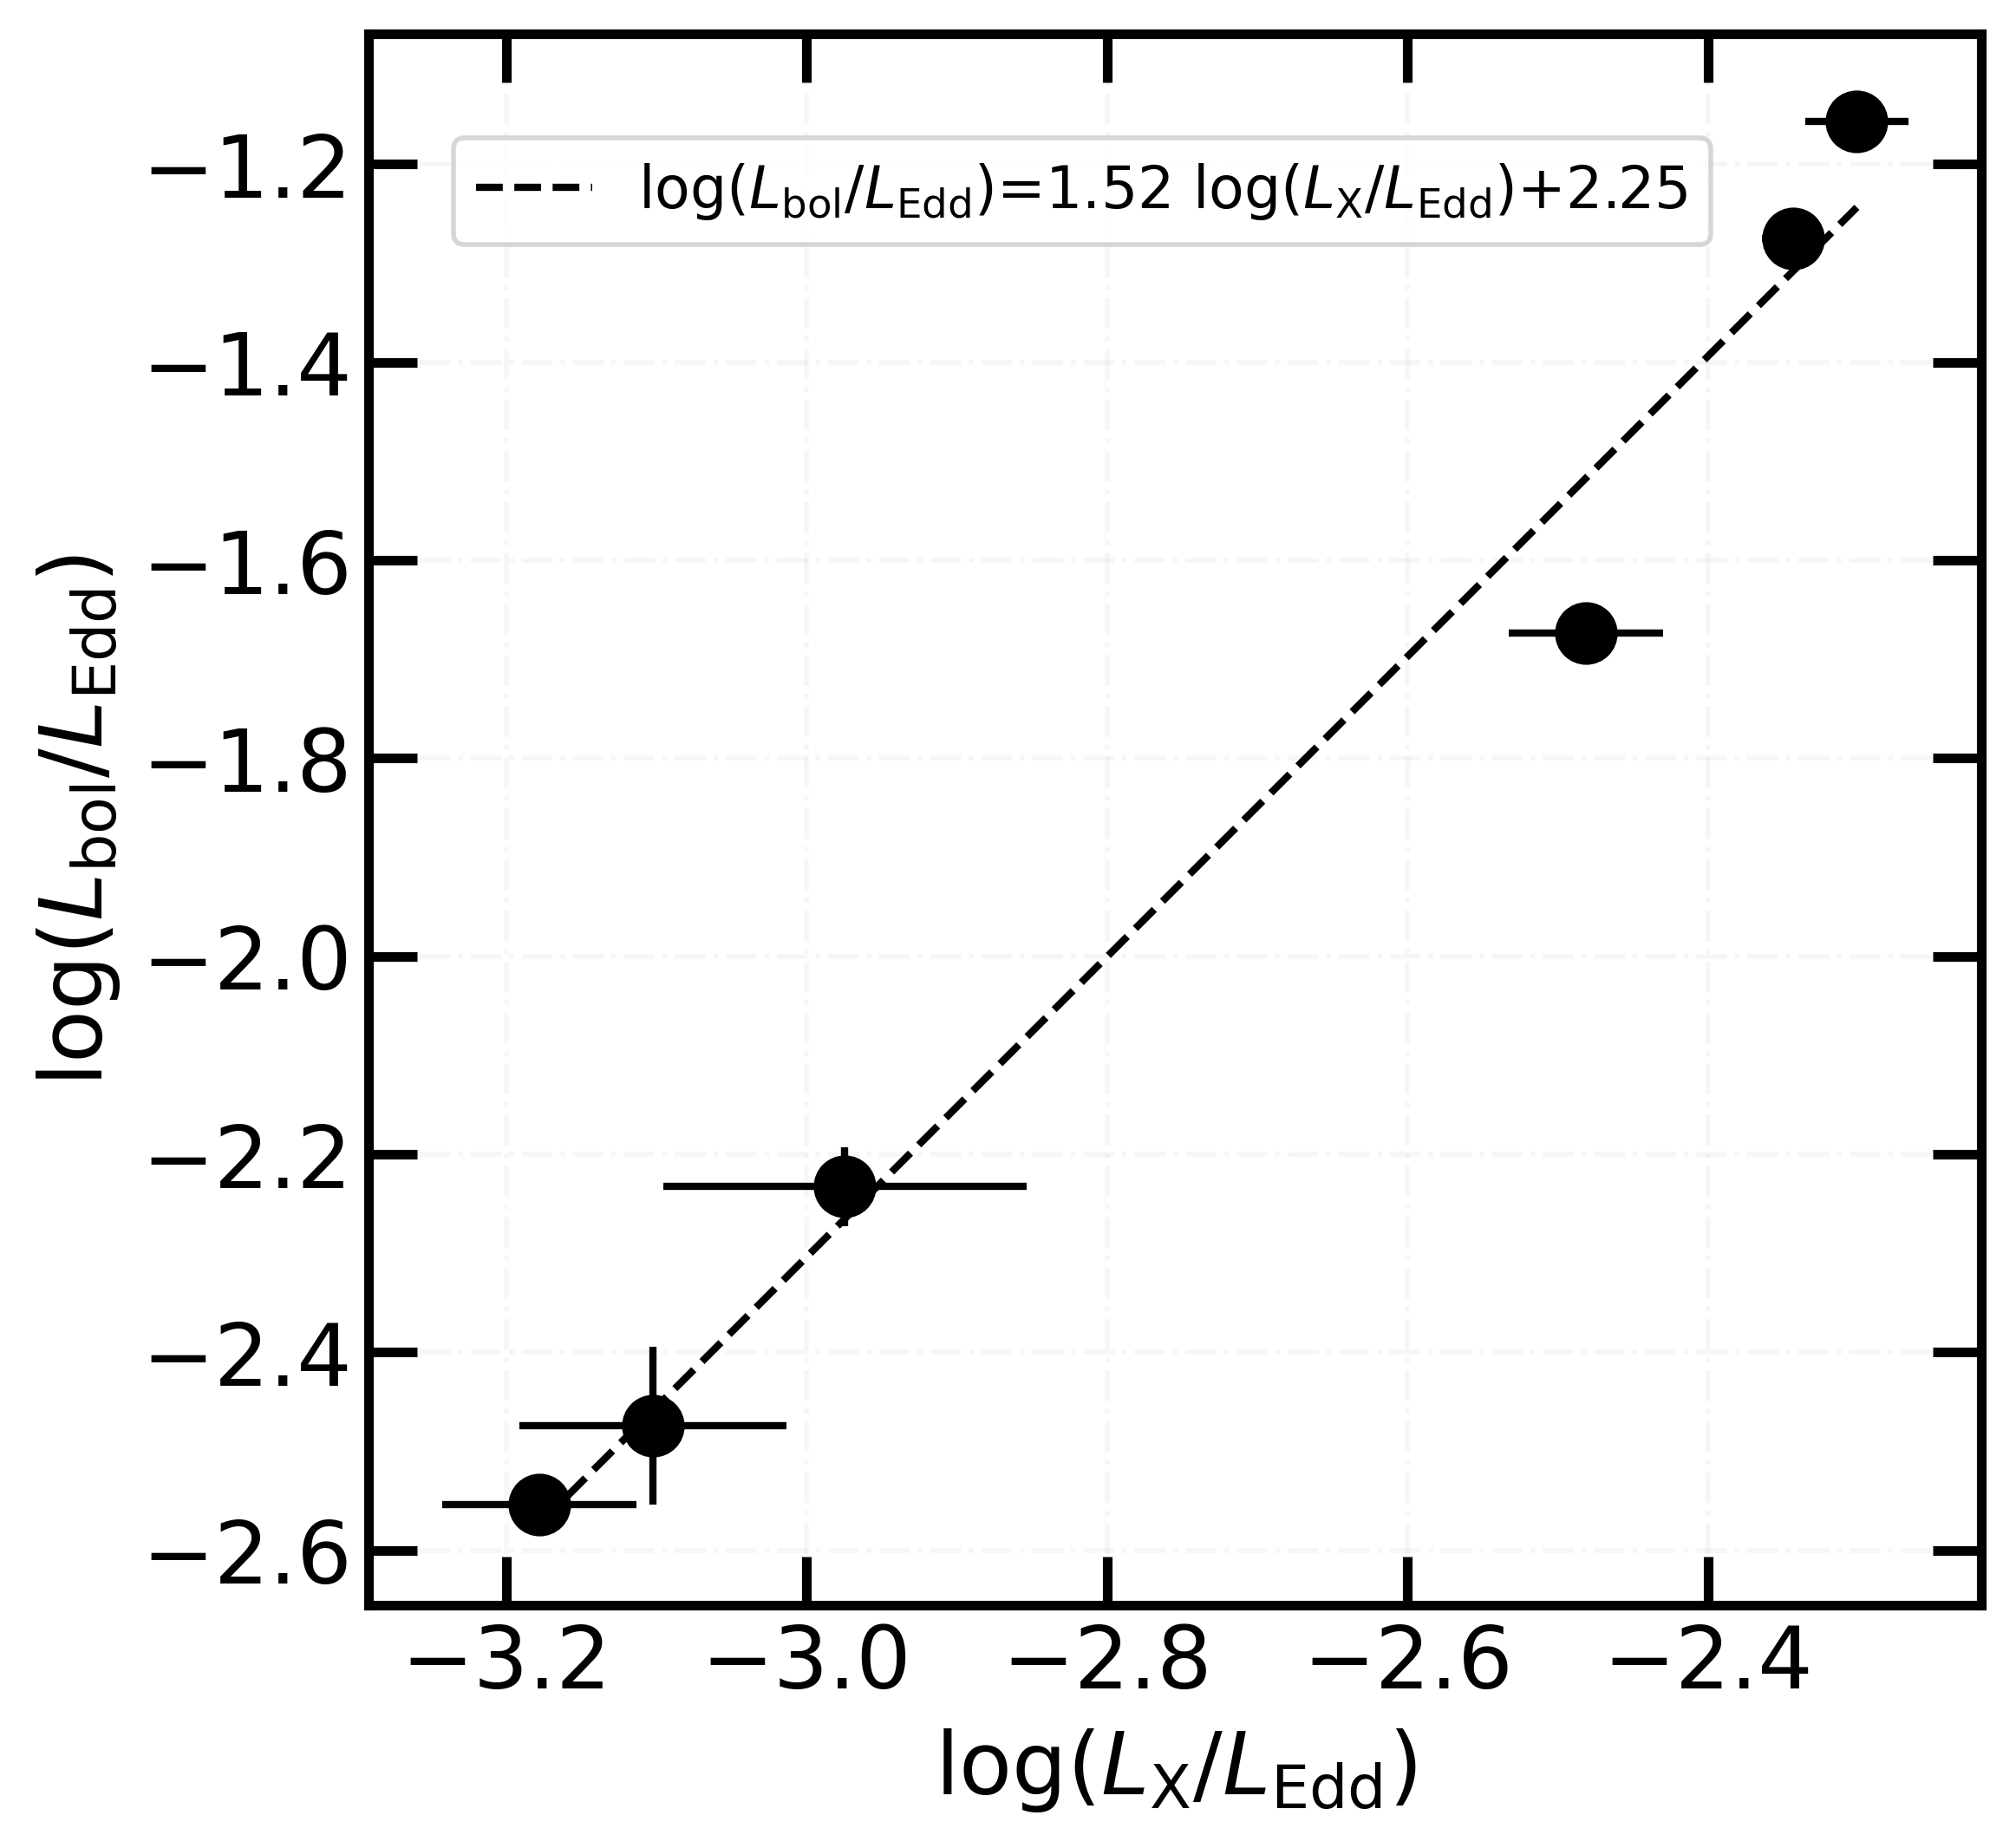
\includegraphics[width=0.6\textwidth]{./pic/Mrk1018_LxvsLBol_fit.png}
    \caption{The $L_\mathrm{bol}/L_\mathrm{Edd}$ - $L_\mathrm{X}/L_\mathrm{Edd}$ correlation.}
    \label{fig:xray-bol}
    %$L_\mathrm{bol}$ is estimated based on the model of \texttt{phabs*redden*(optxagnf+hostpol)}.
    
\end{figure*}

\begin{figure*}
\centering
	% To include a figure from a file named example.*
	% Allowable file formats are eps or ps if compiling using latex
	% or pdf, png, jpg if compiling using pdflatex
	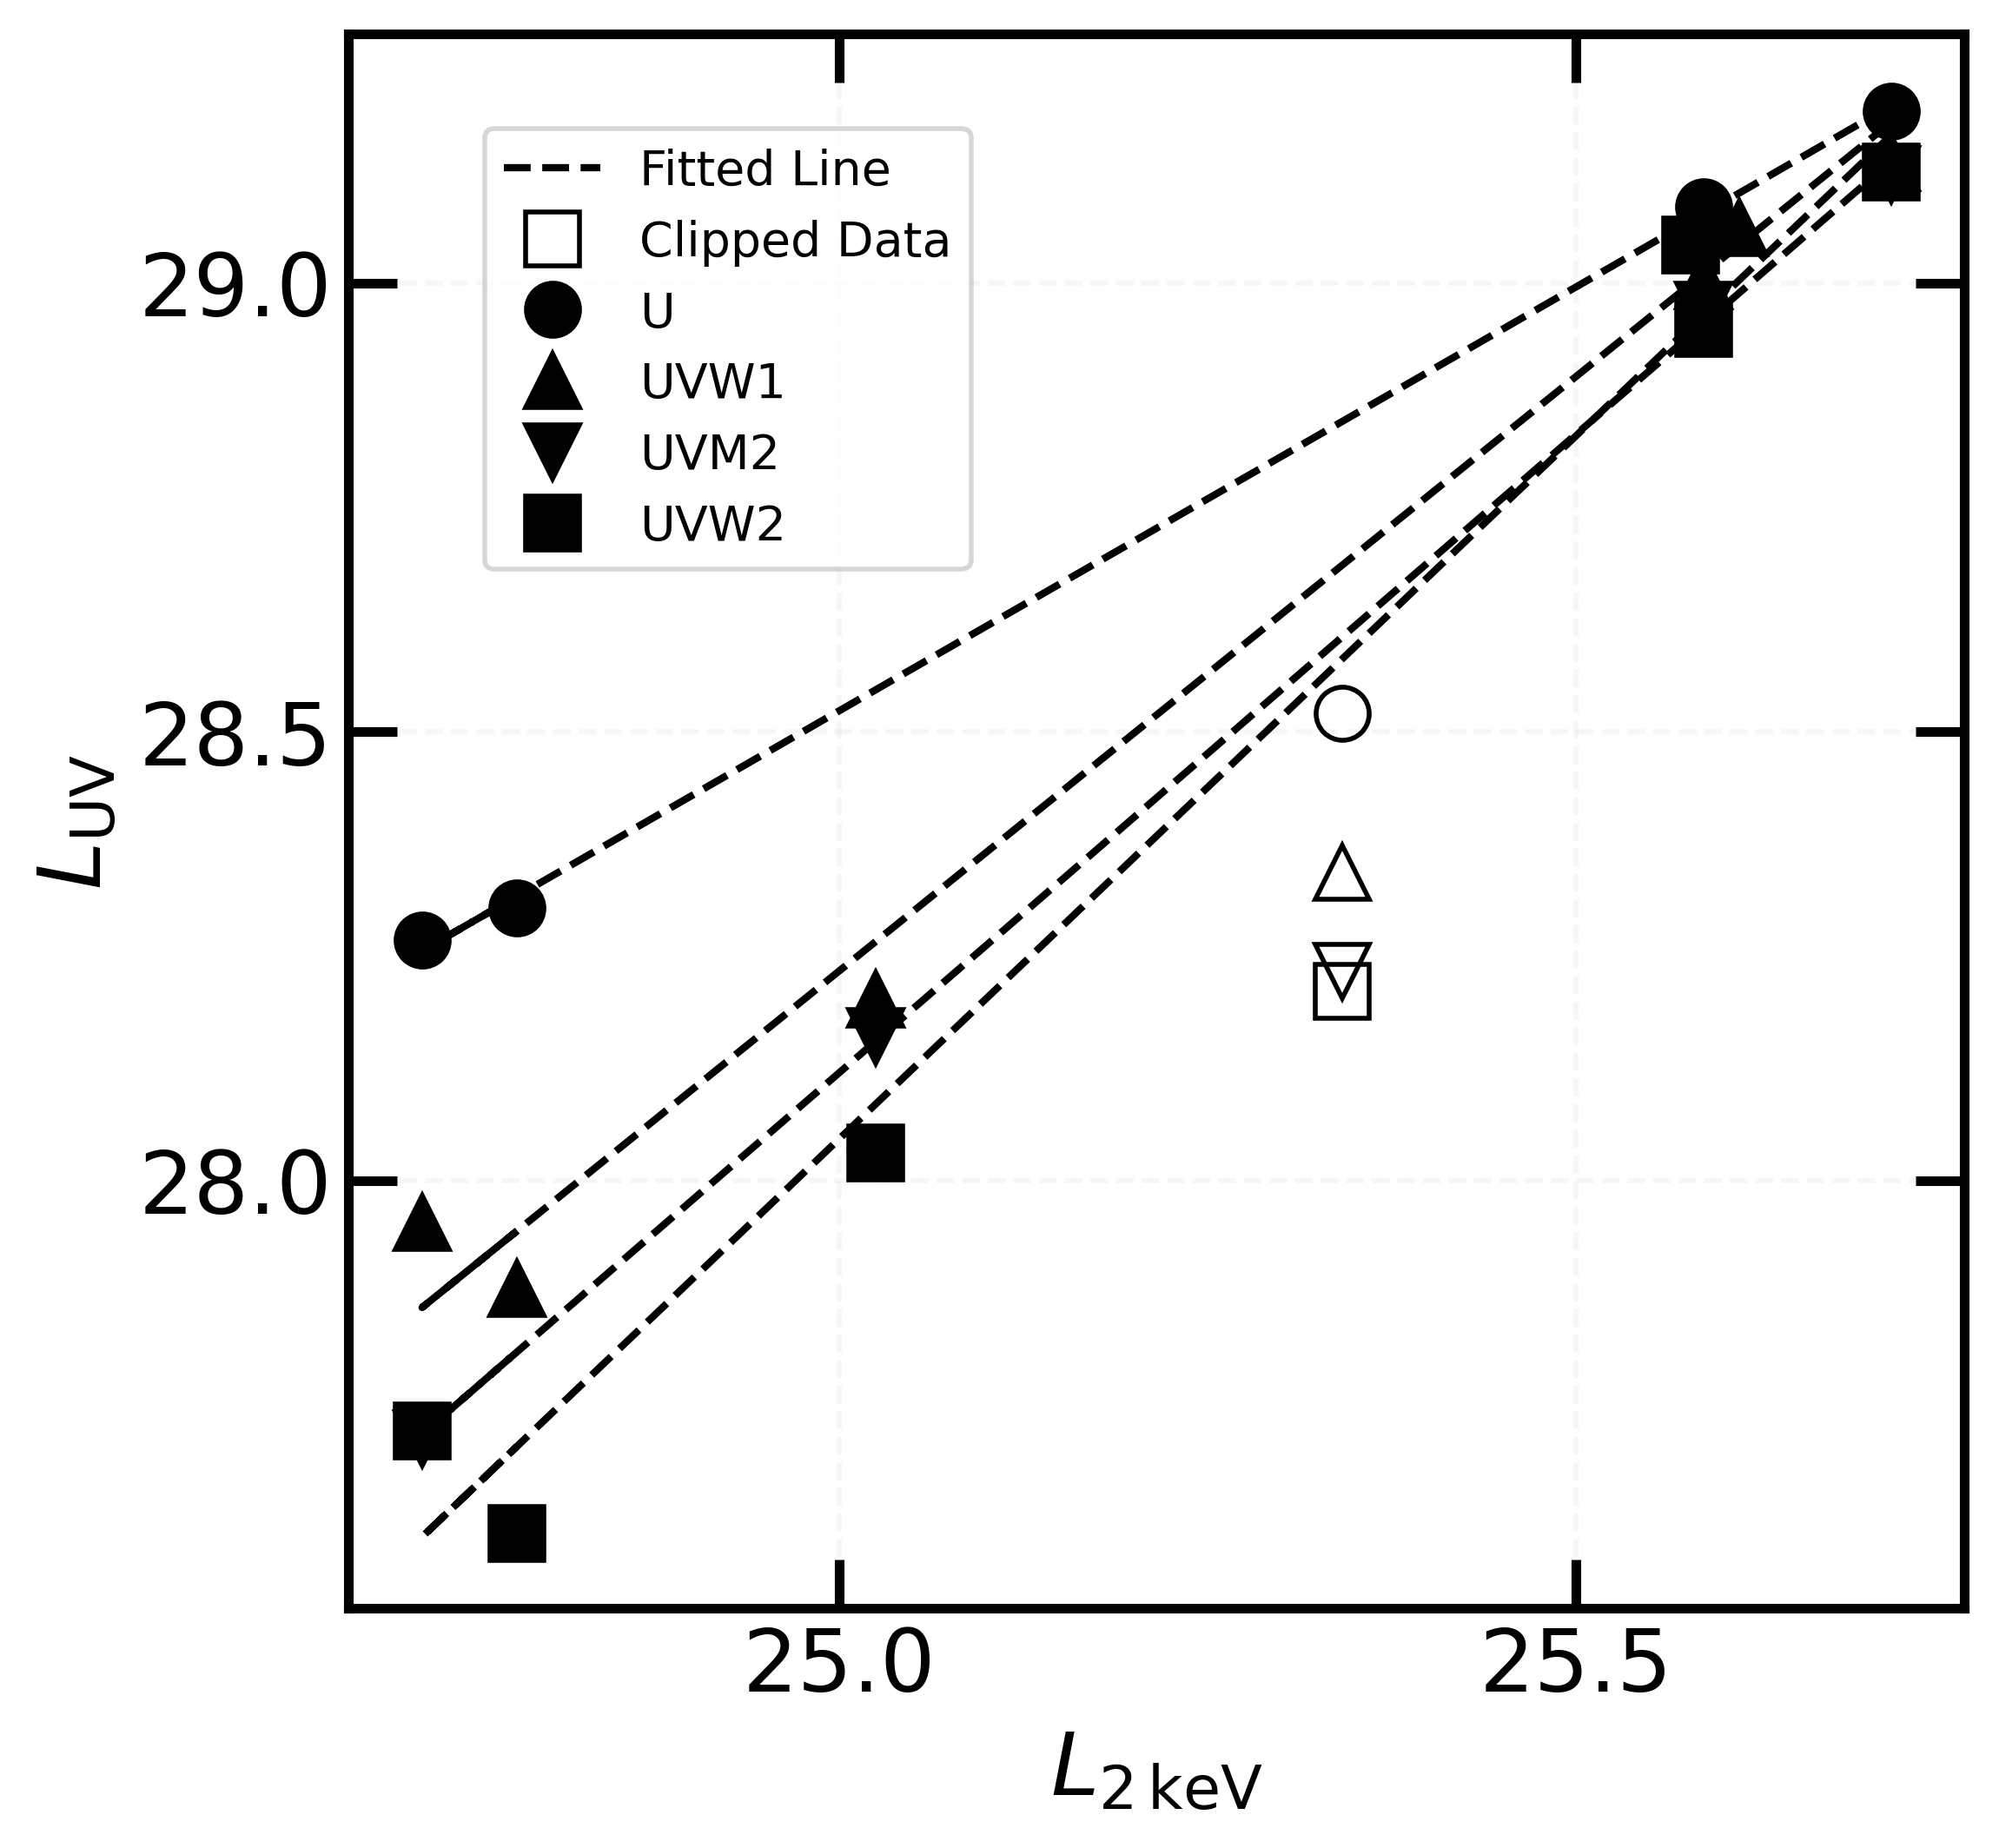
\includegraphics[width=0.6\textwidth]{./pic/Mrk1018_L2_Luvot_correlation-fig-without-outlier_clip.png}
    \caption{The $L_{\nu (\mathrm{UV})}$ - $L_{\nu (\mathrm{2\,keV})}$ correlation during 2005 and 2016. The data in blank markers are regarded as outliers.}
    \label{fig:correlation-Luvot-L2keV}
\end{figure*}


\begin{figure*}
\centering
	% To include a figure from a file named example.*
	% Allowable file formats are eps or ps if compiling using latex
	% or pdf, png, jpg if compiling using pdflatex
	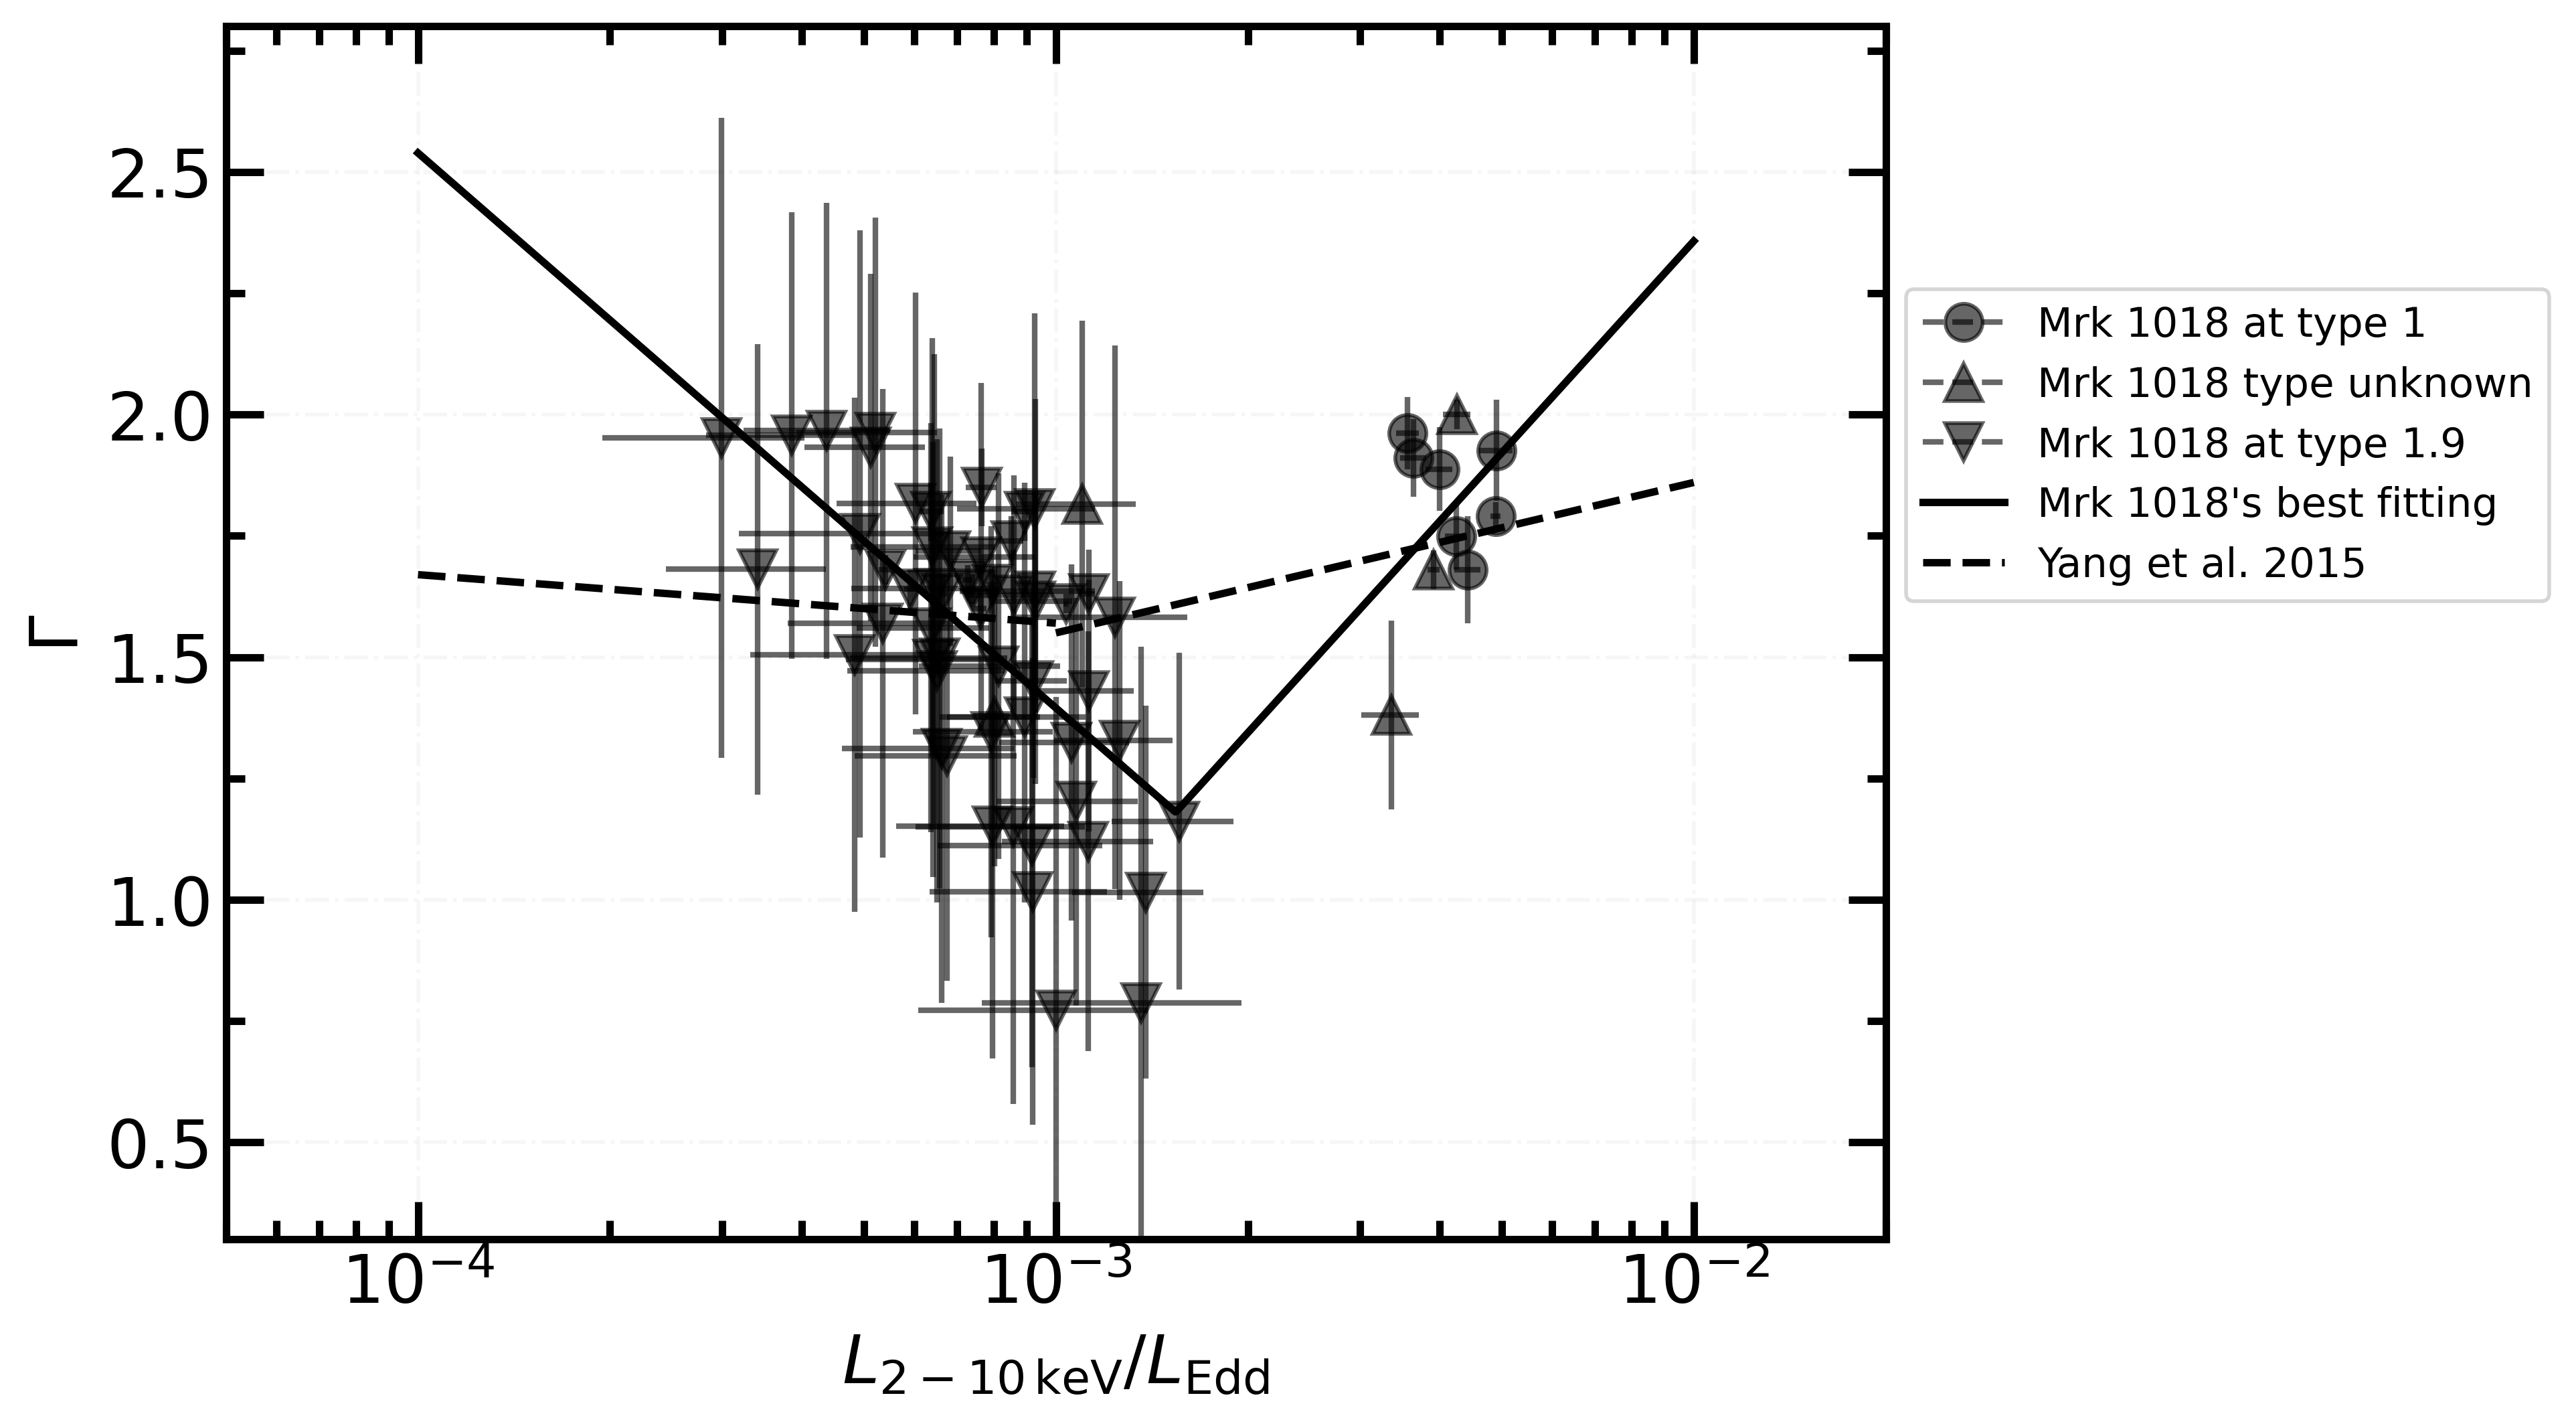
\includegraphics[width=0.7\textwidth]{./pic/xrayappendgood-errorbar-Lrate-g-tmap_brokenlinear_dot.png}
    \caption{The $\Gamma$ - $L_\mathrm{X}/L_\mathrm{Edd}$ correlation with best fitting shown in the broken straight line. The critical $\log(L_\mathrm{X}/L_\mathrm{Edd})$ value is $\sim$ -2.81. The broken dashed line represents the results from \citet{2015MNRAS.447.1692Y} with critical $\log(L_\mathrm{X}/L_\mathrm{Edd})$ value $\sim$ -3. We find a re-flare while Mrk~1018 transited from the left branch to the right branch of $\Gamma$-flux correlation in $\sim$ 98 days and returns to the left branch in $\sim$ 368 days, which are shown in arrows.}
    \label{fig:xrayappendgood-Lrateandg-tmap}
\end{figure*}




\begin{figure*}
\centering
	% To include a figure from a file named example.*
	% Allowable file formats are eps or ps if compiling using latex
	% or pdf, png, jpg if compiling using pdflatex
	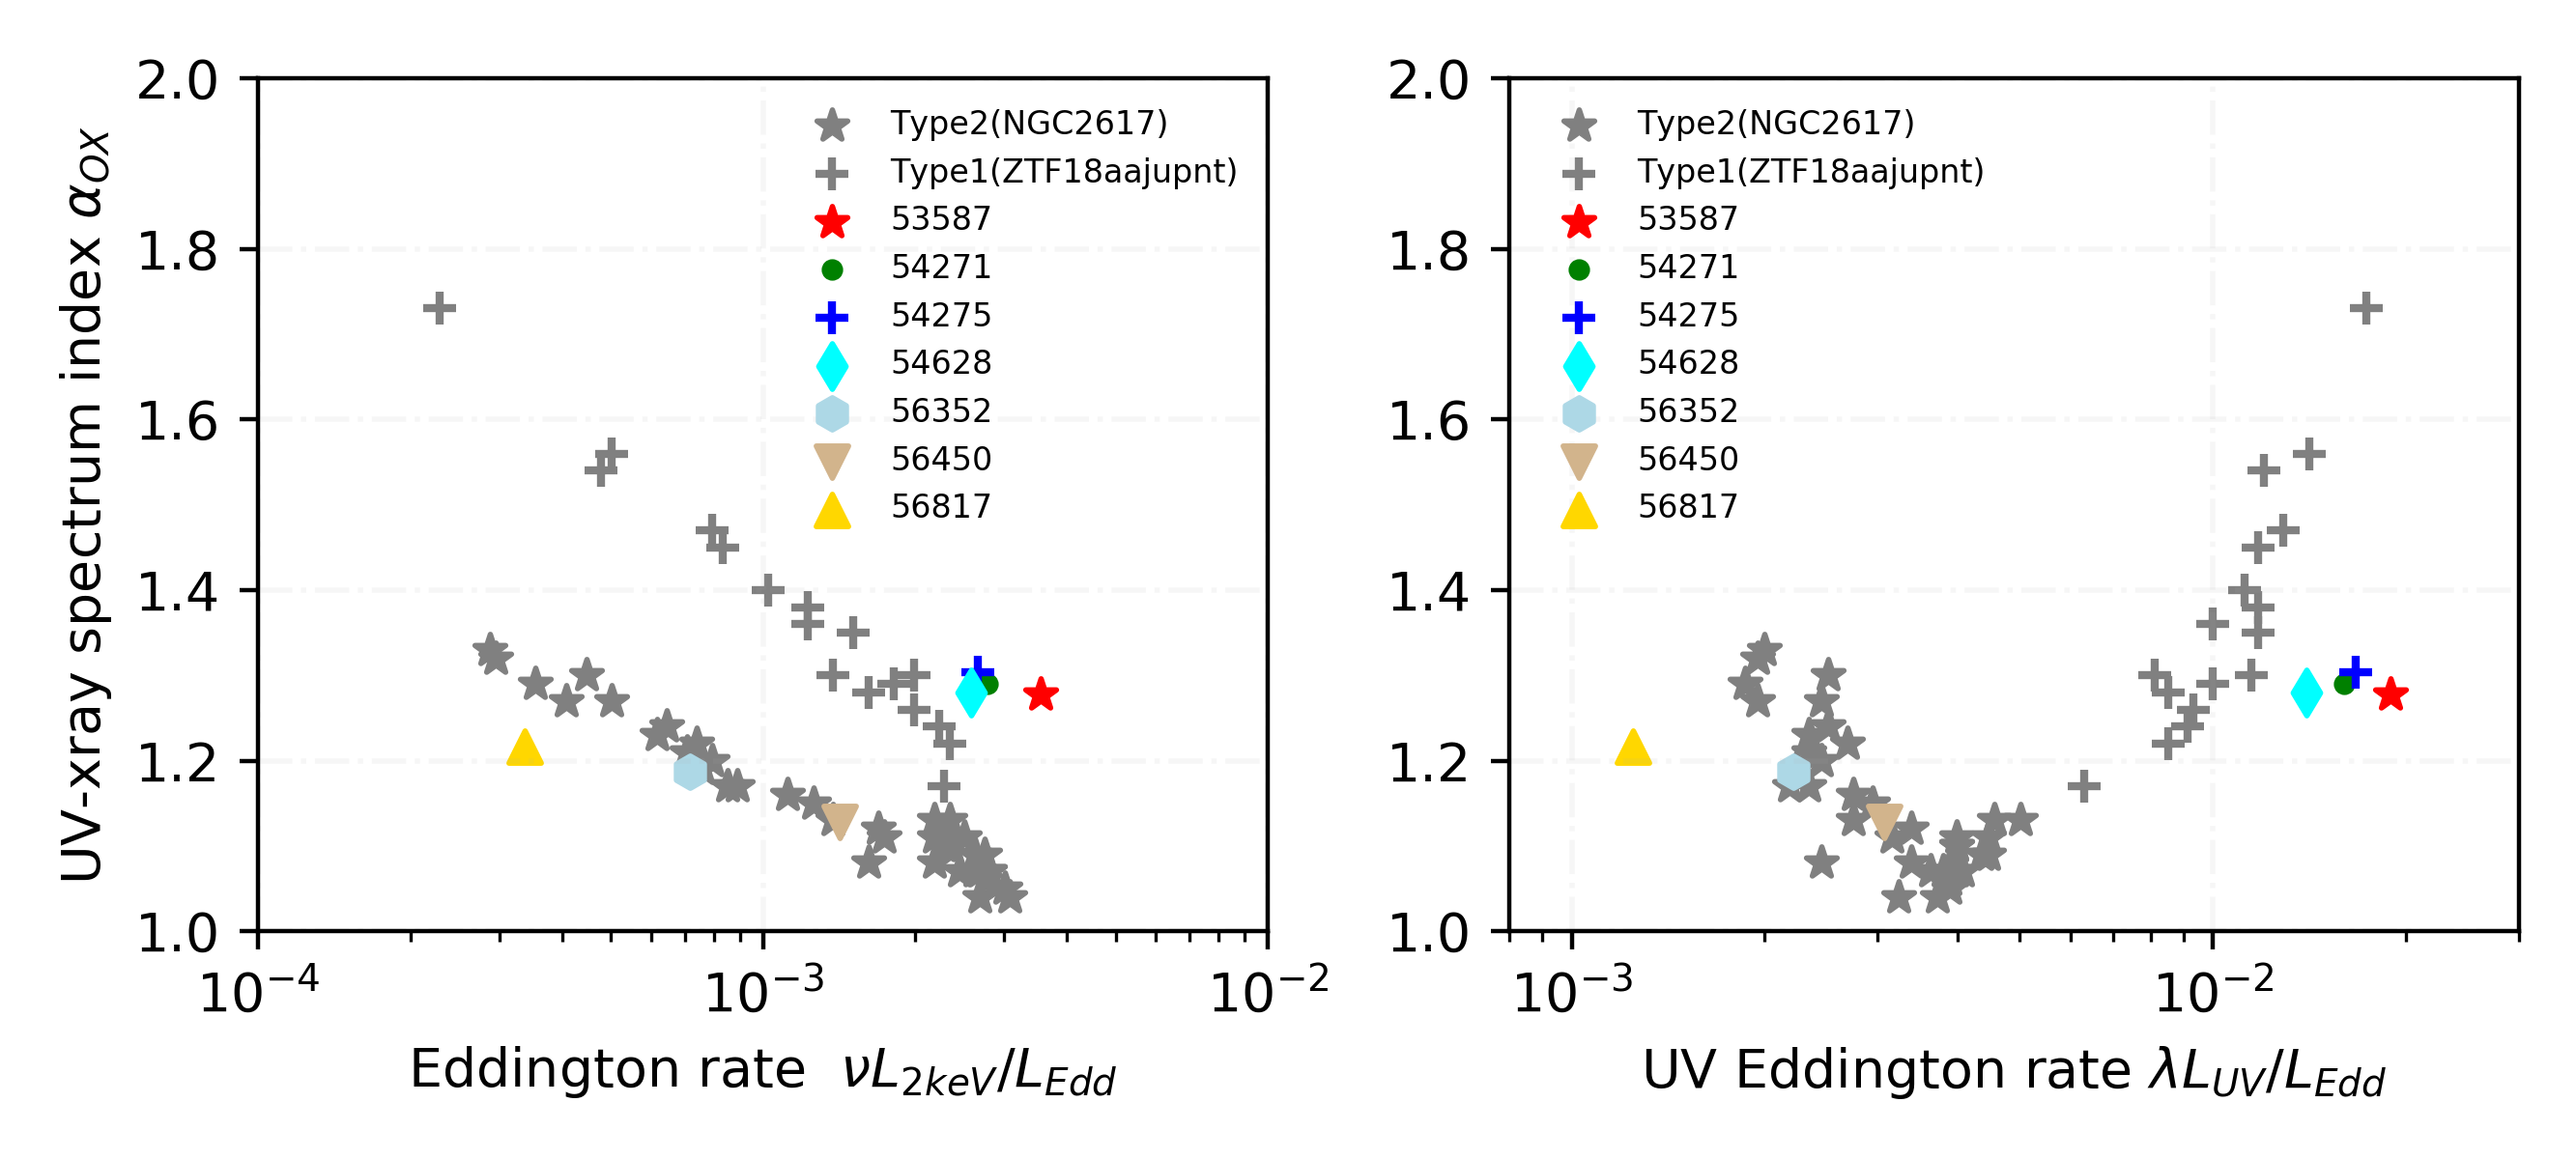
\includegraphics[width=0.9\textwidth]{./pic/Mrk1018_subplots_plus_2individuals_alpha_ox_L_x_Luv_rate.png}
    \caption{The $\alpha_\mathrm{OX}-\nu L_{\nu (\mathrm{2keV})}/L_\mathrm{Edd}$ and $\alpha_\mathrm{OX}-\lambda L_{\nu (\mathrm{UVW1})}/L_\mathrm{Edd}$ correlation in comparison with two CL-AGNs in \citet{2019arXiv190904676R}.}   
    \label{fig:alpha_ox_lx_luv}
\end{figure*}





\begin{figure*}
\centering
	% To include a figure from a file named example.*
	% Allowable file formats are eps or ps if compiling using latex
	% or pdf, png, jpg if compiling using pdflatex
	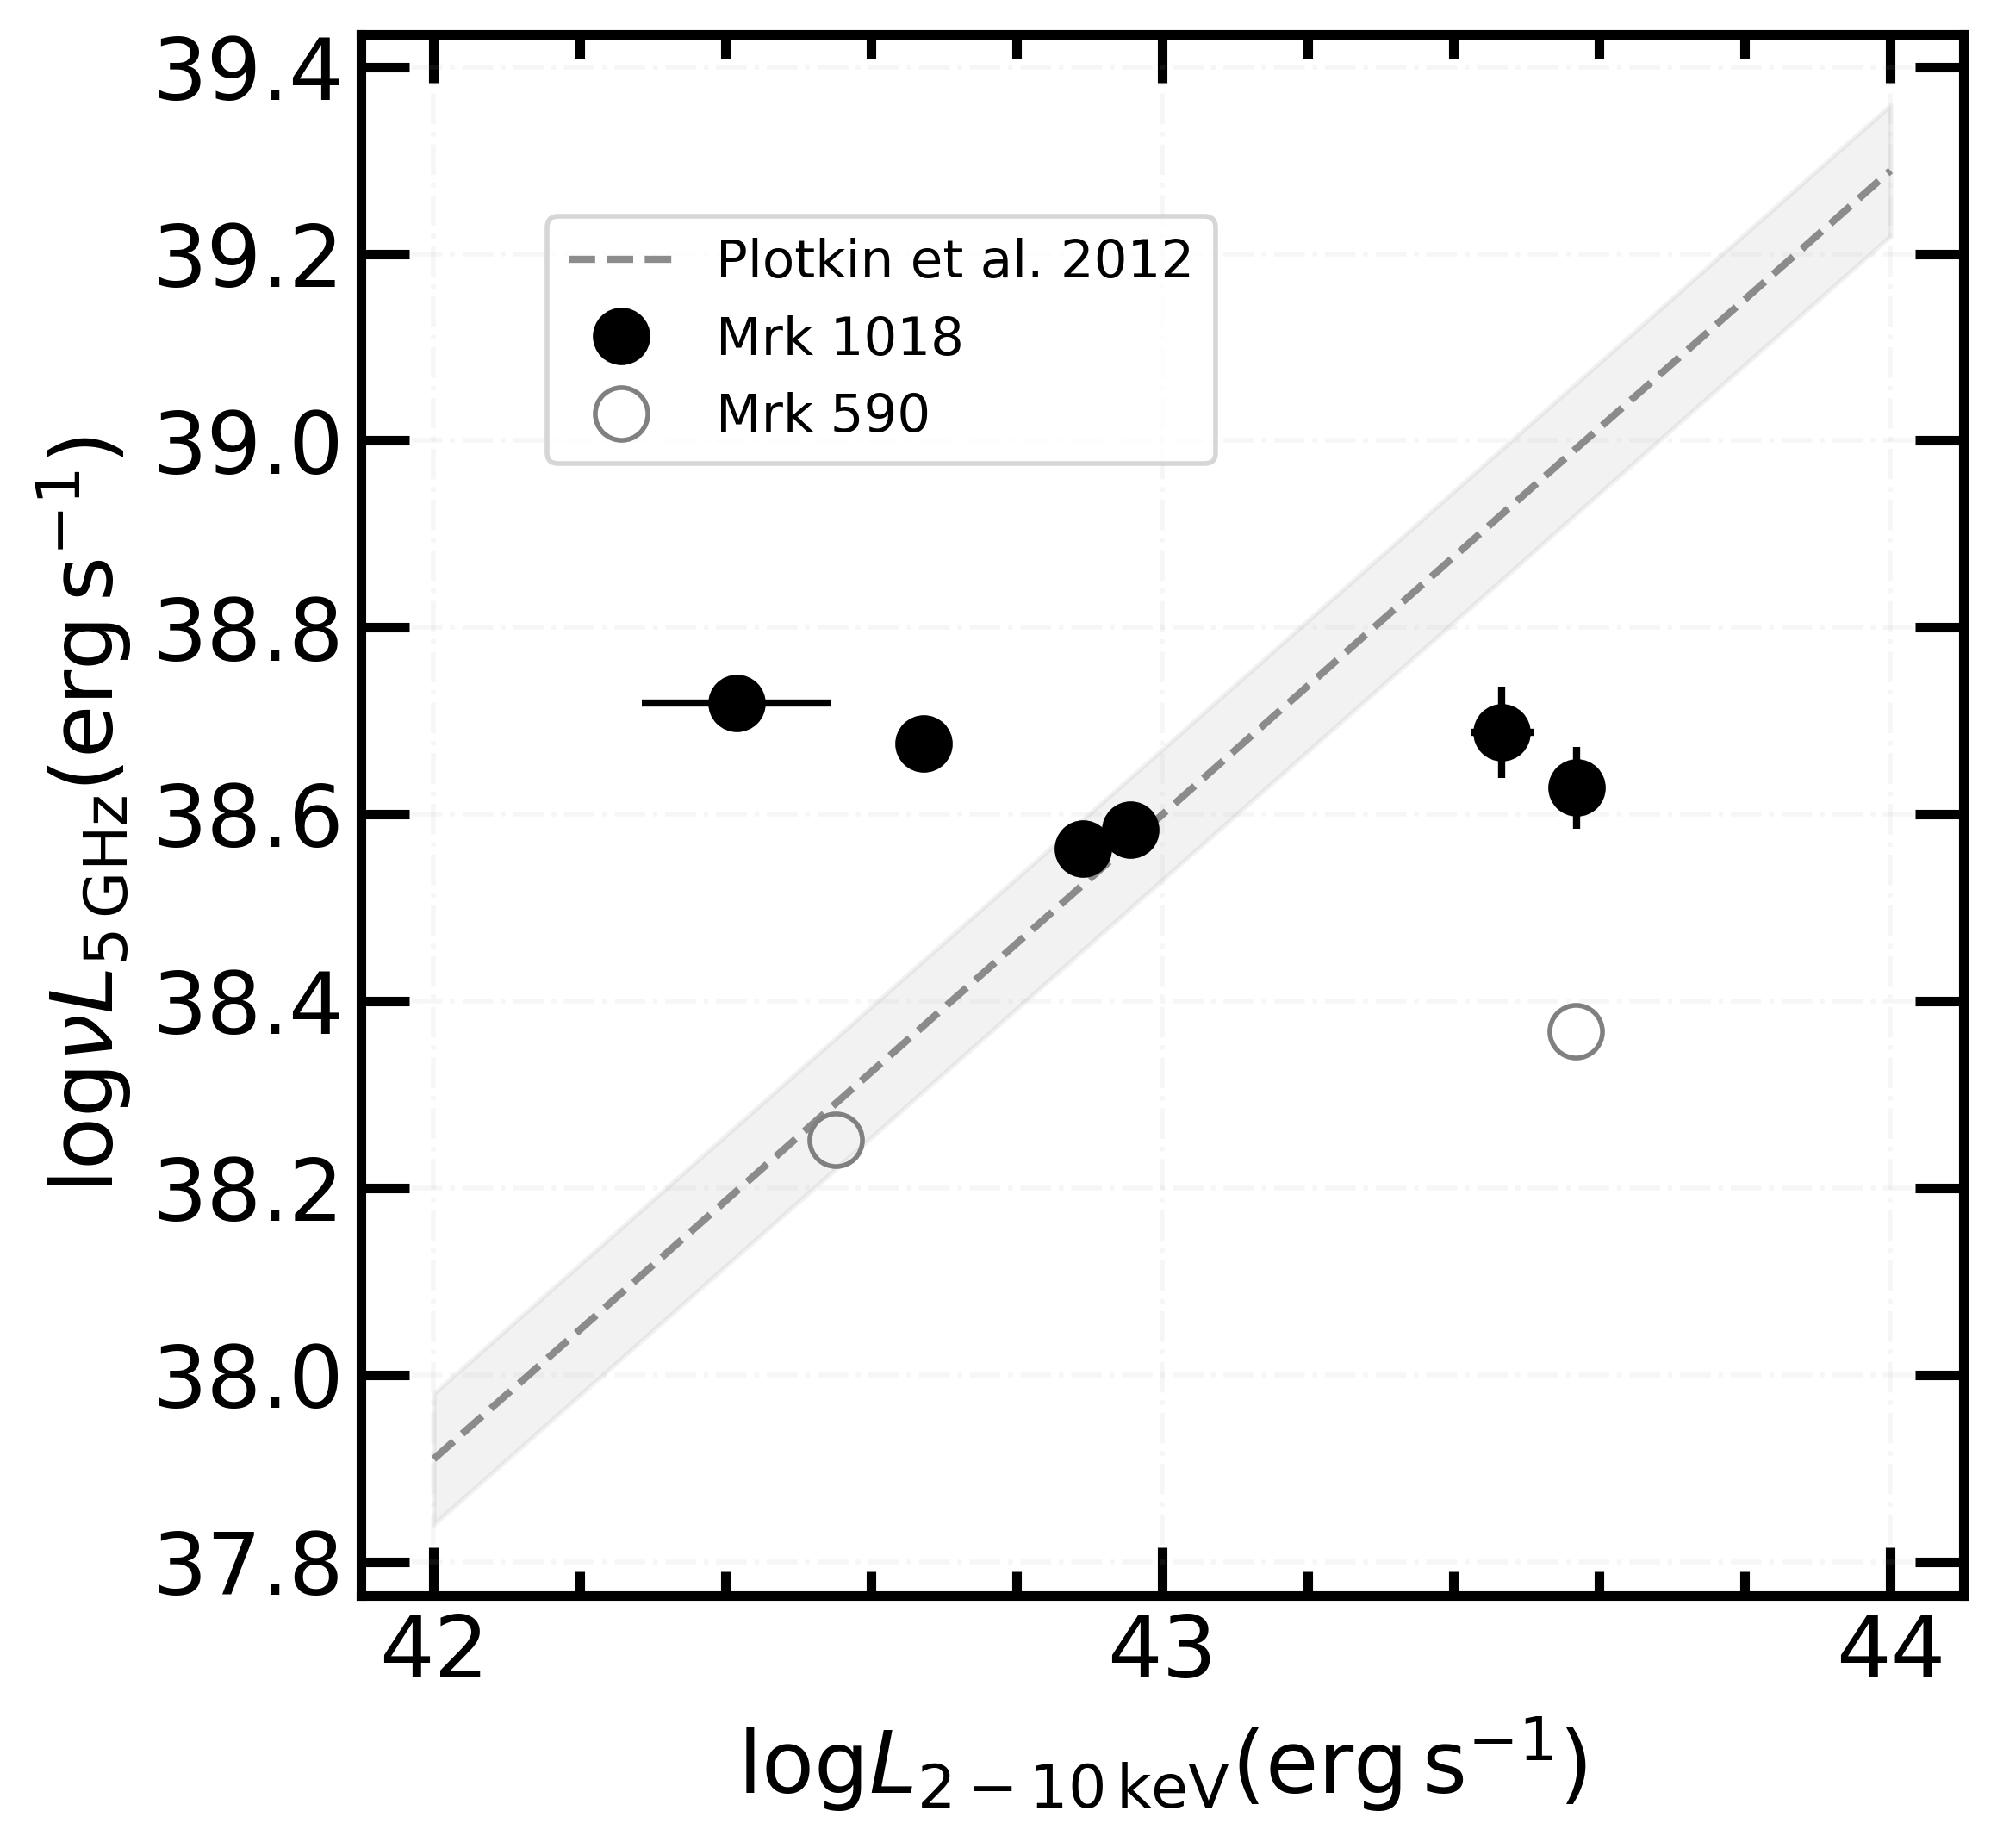
\includegraphics[width=0.6\textwidth]{./pic/Mrk1018_Mrk590_radio_xray_Plotkin2012_Lx.png}
    \caption{The $L_\mathrm{R}$-$L_\mathrm{X}$ relationship relative to fundamental plane defined in \citet{2012MNRAS.419..267P} shown in dashed line with intrinsic $\sigma=0.07$. We add the data of Mrk~590 from Table~5 in \citet{2016MNRAS.460..304K} for comparison.} 
    \label{fig:radio-xray-mass_relation_Plotkin2012}
\end{figure*}



%This work is supported by...
%% To help institutions obtain information on the effectiveness of their 
%% telescopes the AAS Journals has created a group of keywords for telescope 
%% facilities.
%
%% Following the acknowledgments section, use the following syntax and the
%% \facility{} or \facilities{} macros to list the keywords of facilities used 
%% in the research for the paper.  Each keyword is check against the master 
%% list during copy editing.  Individual instruments can be provided in 
%% parentheses, after the keyword, but they are not verified.




%% Appendix material should be preceded with a single \appendix command.
%% There should be a \section command for each appendix. Mark appendix
%% subsections with the same markup you use in the main body of the paper.

%% Each Appendix (indicated with \section) will be lettered A, B, C, etc.
%% The equation counter will reset when it encounters the \appendix
%% command and will number appendix equations (A1), (A2), etc. The
%% Figure and Table counter will not reset.

\clearpage
%\bibliographystyle{mnras}
\bibliography{refMrk1018}{}
% if your bibtex file is called example.bib
\bibliographystyle{aasjournal}
%\clearpage

\begin{table}
\centering
\caption{{ \bf X-ray fit parameters of Mrk~1018. } Columns include the date of the observation, the facility, observation id, reduced $\chi ^2$ of the best fit model, the photon index $\Gamma$ with 90\% uncertainty, and the flux in 2-10~keV after Galactic-absorption correction. }
\label{tab:table1}

\begin{tabular}{lcccccc}
\hline
\hline
 
  Date   &   Instrument & obsid  & $\chi ^2$  &$\Gamma$  &  $F_{2-10keV}$  & \\ 
  (MJD)  &              &        &          &                    &  [erg cm$^{-2}$ s$^{-1}$] &      
 \\  \hline
53385 & X & 201090201 & 0.98 & 1.73 $\pm$ 0.07 & 9.7e-12 $\pm$ 6e-13 \\ 
53587 & S & 35166001 & 0.78 & 1.93 $\pm$ 0.1 & 1.15e-11 $\pm$ 6.99e-13 \\ 
54271 & S & 30955001 & 1.01 & 1.89 $\pm$ 0.09 & 9.39e-12 $\pm$ 4.47e-13 \\ 
54274 & S & 30955002 & 1.07 & 1.91 $\pm$ 0.08 & 8.54e-12 $\pm$ 4e-13 \\ 
54276 & S & 30955003 & 1.02 & 1.96 $\pm$ 0.08 & 8.38e-12 $\pm$ 3.47e-13 \\ 
54628 & S & 35776001 & 1.19 & 1.75 $\pm$ 0.07 & 9.98e-12 $\pm$ 3.96e-13 \\ 
54685 & X & 554920301 & 1.16 & 1.79 $\pm$ 0.02 & 1.13e-11 $\pm$ 2e-13 \\ 
55527$^{(a)}$ & C & 12868 & 1.1 & 1.7 $\pm$ 0.03 & 9.26e-12 $\pm$ 1.9e-13 \\ 
56353 & S & 49654001 & 1.42 & 1.82 $\pm$ 0.38 & 2.59e-12 $\pm$ 5.52e-13 \\ 
56450 & S & 49654002 & 1.23 & 1.38 $\pm$ 0.19 & 7.9e-12 $\pm$ 8.21e-13 \\ 
56818 & S & 49654004 & 0.75 & 1.38 $\pm$ 0.31 & 1.88e-12 $\pm$ 3.37e-13 \\ 
57428 & N & 60160087002 & 1.23 & 1.85 $\pm$ 0.08 & 1.8e-12 $\pm$ 1e-13 \\ 
57429 & S & 80898001 & 0.96 & 1.72 $\pm$ 0.2 & 1.61e-12 $\pm$ 1.89e-13 \\ 
57434 & S & 80898002 & 0.9 & 1.45 $\pm$ 0.2 & 2.17e-12 $\pm$ 2.77e-13 \\ 
57443 & C & 18789 & 0.82 & 1.7 $\pm$ 0.03 & 1.3e-12 $\pm$ 3e-14 \\ 
57801 & C & 19560 & 1.26 & 1.61 $\pm$ 0.02 & 2.48e-12 $\pm$ 4e-14 \\ 
58123 & N & 60301022002 & 1.34 & 1.8 $\pm$ 0.06 & 2.1e-12 $\pm$ 1e-13 \\ 
58125 & S & 88207001 & 1.04 & 1.63 $\pm$ 0.25 & 2.02e-12 $\pm$ 3.08e-13 \\ 
58126 & C & 20366 & 1.05 & 1.6 $\pm$ 0.03 & 1.84e-12 $\pm$ 5e-14 \\ 
58180 & C & 20367 & 1.02 & 1.61 $\pm$ 0.04 & 1.59e-12 $\pm$ 5e-14 \\ 
58182 & N & 60301022003 & 1.03 & 1.8 $\pm$ 0.06 & 1.5e-12 $\pm$ 7e-14 \\ 
58281 & C & 20368 & 1.02 & 1.62 $\pm$ 0.03 & 1.77e-12 $\pm$ 5e-14 \\ 
58316 & N & 60301022005 & 0.85 & 1.74 $\pm$ 0.05 & 2e-12 $\pm$ 9e-14 \\ 
58317 & S & 88207003 & 1.01 & 1.61 $\pm$ 0.23 & 2.18e-12 $\pm$ 3.12e-13 \\  \\ \hline
\end{tabular}\\
Notes: Here the superscripts $^{(a)}$ represents fit result that are taken from \citet{2017A&A...607L...9K}. Instrument indicate by C-\chandra, S-\swift, X-\xmm, N-\nustar. 
\end{table}
\clearpage
%






\begin{table}
\centering
\caption{{\bf $\alpha_{ox}$ of Mrk~1018 with simultaneous XRT and UVOT observation.} Columns include the date of the observation, $\alpha_{ox}$, flux in 2-10~keV, $\nu F_{uw1}$, and Eddington rate.}
\label{tab:tablealpha_ox}
\begin{tabular}{lcccccc}
\hline
\hline
 
 Date &   $\alpha_{ox}$  & $F_{2-10keV}$  &$\nu F_{uw1}$  & $L_{2-10keV}/L_{Edd}$ &   $\nu L_{uw1}/L_{Edd}$  \\ 
 (MJD)&                   &   [erg cm$^{-2}$ s$^{-1}$]   &[erg cm$^{-2}$ s$^{-1}$]    &                    &            
 \\ \hline
53587 & 1.29 & 1.14e-11 & 3.92e-11 & 5.53e-03 & 1.90e-02 \\ 
54271 & 1.30 & 9.34e-12 & 3.31e-11 & 4.51e-03 & 1.60e-02 \\ 
54275 & 1.31 & 8.78e-12 & 3.45e-11 & 4.24e-03 & 1.67e-02 \\ 
54628 & 1.29 & 9.85e-12 & 2.89e-11 & 4.76e-03 & 1.40e-02 \\ 
56352 & 1.20 & 2.59e-12 & 4.58e-12 & 1.25e-03 & 2.22e-03 \\ 
56450 & 1.14 & 8.26e-12 & 6.35e-12 & 3.99e-03 & 3.07e-03 \\ 
56817 & 1.23 & 1.98e-12 & 2.58e-12 & 9.57e-04 & 1.25e-03 \\ \hline
\end{tabular}   
\end{table}
\begin{table}
\centering
\caption{{\bf VLA observation of Mrk~1018.} Columns include the date of observation, project name, band, frequency, integrated flux, radio spectral index ($\alpha$) and reference.}
\label{tab:tableradio}
\begin{tabular}{lcccccr}
\hline
\hline
 
 Date &  project & band  & Frequency  &$F_{int}$   & $\alpha$ & Reference  \\ 
 (MJD)&         &        &   [GHz]   &[mJy]     &                &         \\ \hline
    \multirow{2}*{46032} & \multirow{2}*{AU0020} & L    & 1.49  & 4.21  $\pm$ 0.23  & \multirow{2}*{0.52 $\pm0.07$} &\\
    \,          &        & C     & 4.86  & 2.29  $\pm$ 0.14  & & \\
    47261     & AB0476 & C     & 4.86  & 1.91  $\pm$ 0.23  &  &\\
    47692     & AB0540A & C     & 4.86  & 2.62  $\pm$ 0.16  &  &\\
    47732     & AB0540B & C     & 4.86  & 2.31  $\pm$ 0.17  & & \\
    49820.5 $\pm$ 773.5 & AB0628 & L     & 1.4   & 4.20  $\pm$ 0.45  &  & \citet{1998AJ....115.1693C} \\
    49820.5 $\pm$ 773.5 & AB0628 & L     & 1.4   & 4.15  $\pm$ 0.25  &  & \citet{1997ApJ...475..479W} \\
    50219.5 $\pm$ 1078.5 & AB0308 & L     & 1.4   & 4.20  $\pm$ 0.54  &  & \citet{2002AJ....124..675C}\\
    50970     & AB0878 & X     & 8.46  & 2.47  $\pm$ 0.17  & 0.3 $\pm0.08$\\
    52246.5 $\pm$ 278.5 & AB0950 & L     & 1.4   & 4.15  $\pm$ 0.25  & & \citet{2003yCat.8071....0B} \\
    54872.5 $\pm$ 51.5  & AR685 & L     & 1.4   & 3.69  $\pm$ 0.19  &  & \citet{2011AJ....142....3H}\\
    54878   & AB1314 & L     & 1.4   & 3.36  $\pm$ 0.20  &  & \citet{2012yCat.8090....0B} \\
    56550 $\pm$ 8     & 13B-272 & L     & 1.4   & 3.85  $\pm$ 0.31  &  & \citet{2016MNRAS.460.4433H} \\

    \multirow{3}*{57481}     &  \multirow{3}*{16A-444} & C     & 5     & 2.56  $\pm$ 0.13  & \multirow{3}*{0.02$\pm0.05$}& \\
              &     & X     & 10    & 2.16  $\pm$ 0.11  & &\\
              &    &  K     & 22    & 2.46  $\pm$ 0.12  &  &\\
    57719     & 16B-084 & X     & 10    & 1.78  $\pm$ 0.09  &   &\\

    57731     & 16B-084 & X     & 10    & 1.97  $\pm$ 0.10  &  &\\

    57768     & 16B-084 & C     & 5     & 2.07  $\pm$ 0.10  & 0 &\\
    58087     & VLASS1.1 & L     & 3     & 2.30  $\pm$ 0.36  & & \\
    
    58472     & 18B-245 & K     & 20    & 2.71  $\pm$ 0.14  &  & \\



\hline 
\end{tabular}   
\end{table}




     
\begin{table}
\centering
\caption{{\bf Radio and X-ray luminosity diagram.} Columns include the date of the radio observation, the radio spectrum index $\alpha_{radio}$, the date of X-ray observation, the interval between two bands, the flux and luminosity rescaled to 4.8 and 8.4~GHz, the X-ray flux and luminosity in 2-10~keV band.}
\label{tab:table4}
\begin{tabular}{lllllllllr}
\hline
\hline

$T_{Radio}$ &  $\alpha_{Radio}$ & $T_{X-ray}$ & $\delta$ T & $F_{2-10keV}$ & $F_{4.8GHz}$ & $F_{8.4GHz}$ &  $\nu L_{\nu=4.8GHz}$ &  $\nu L_{\nu=8.4GHz}$ & $L_{\rm{2--10~keV}}$ \\ 
(MJD)  &  & (MJD)  &(day)  &[erg$~s^{-1}~\rm{cm}^{-2}$] & [mJy)& (mJy)]& [erg$~s^{-1} $] & [erg$~s^{-1} $]& [erg$~s^{-1} $]\\
\hline

52246.5 & 0.42 & 53385 & 1138 & 9.70e-12 & 2.47 & 1.96 & 5.00e38 & 6.92e38 & 4.09e43 \\ 
54318 & 0.42 & 54276 & 42 & 8.78e-12 & 2.00 & 1.58 & 4.05e38 & 5.60e38 & 3.70e43 \\ 
54872.5 & 0.42 & 54685 & 188 & 1.13e-11 & 2.20 & 1.74 & 4.45e39 & 6.15e39 & 4.76e44 \\ 
56550 & 0.42 & 56450 & 100 & 8.26e-12 & 2.29 & 1.81 & 4.64e40 & 6.42e40 & 3.48e45 \\ 
57481 & 0.17 & 57443 & 38 & 1.30e-12 & 2.49 & 2.27 & 5.04e41 & 8.02e41 & 5.48e45 \\ 
57768 & 0.17 & 57801 & 33 & 2.48e-12 & 2.00 & 1.82 & 4.05e42 & 6.45e42 & 1.04e47 \\  \hline
\end{tabular}\\
Notes: We assume the $\alpha_{Radio}$ before/after the type transition as a constant, respectively. 
\end{table}


%\appendix
%\section{Appendix}


%\clearpage


%\clearpage


%% For this sample we use BibTeX plus aasjournals.bst to generate the
%% the bibliography. The sample63.bib file was populated from ADS. To
%% get the citations to show in the compiled file do the following:
%%
%% pdflatex sample63.tex
%% bibtext sample63
%% pdflatex sample63.tex
%% pdflatex sample63.tex




%% This command is needed to show the entire author+affiliation list when
%% the collaboration and author truncation commands are used.  It has to
%% go at the end of the manuscript.
%\allauthors

%% Include this line if you are using the \added, \replaced, \deleted
%% commands to see a summary list of all changes at the end of the article.
%\listofchanges
% Don't change these lines
%\bsp	% typesetting comment
%\label{lastpage}
\end{document}

% End of file `sample63.tex'.
